%:Clase del documento
\documentclass[fontsize=10pt, Myfinal=true, English=true, twoside, numbers=noenddot]{scrbook}
%Minion=true, English=true, Myfinal=true

\makeatletter
\let\alloc@latex\alloc@
\def\alloc@#1#2#3#4{\newcount}% the current \newcount doesn't use \alloc@
\makeatother


%:Paquete de estilos propuesto
\usepackage{libroETSI}
%:Paquete específico para cargar tikz (y sus librerías) y pgfplots
\usepackage{dtsc-creafig}
%:Paquete para notaciones específicas
\usepackage{notacion}
%:Paquete para incorporar aspectos concretos de la edición
\usepackage{edicionPFC}


\makeatletter
\let\alloc@\alloc@latex
\makeatother


%:Estas líneas de código son INNECESARIAS excepto para mostrar determinadas características en este manual. Pueden eliminarse o comentarse sin ningún problema.
%Se usan para compilar el capítulo estilolibroetsi.tex
\usepackage[final]{showexpl}
\lstset{explpreset={frame=none,rframe={}, numbers=none,numbersep=3pt, columns=flexible,language={[LaTeX]TeX},basicstyle=\ttfamily,keywordstyle=\color{blue}}}%numberstyle=\tiny,

%:Para modificar fácilmente la fuente del texto.
\makeatletter
\ifdtsc@Minion % Queremos utilizar la fuente Minion y lo hemos declarado al principio
	\ifluatex
		\setmainfon$•$t[Renderer=Basic, Ligatures=TeX,	% Fuente del texto 
		Scale=1.01,
		]{Minion Pro}
   		% En este caso conviene modificar ligeramente el tamaño de las fuentes matemáticas
		\DeclareMathSizes{10}{10.5}{7.35}{5.25}
		\DeclareMathSizes{10.95}{11.55}{8.08}{5.77}
		\DeclareMathSizes{12}{12.6}{8.82}{6.3}
%		\setmainfont[Renderer=Basic, Ligatures=TeX,	% Fuente del texto 
%		]{Adobe Garamond Pro}
%		\setmainfont[Renderer=Basic, Ligatures=TeX,	% Fuente del texto 
%		]{Palatino LT Std}
	\fi
\else
	\ifluatex
		% Para utilizar la fuente Times New Roman, o alguna otra que se tenga instalada
		\setmainfont[Renderer=Basic, Ligatures=TeX,	% Fuente del texto 
		Scale=1.0,
		]{Times New Roman}
	\else
		\usepackage{tgtermes} 	%clone of Times
		%\usepackage[default]{droidserif}
		%\usepackage{anttor} 	
	\fi
\fi
\makeatother

%Por si quieren usar bibliografía con BIBER
%BIBER%%:Para la bibliografía en BIBER, descomentar las líneas siguientes
%\defbibheading{etsi}[]{%
%	\chapter*{Bibliografía}%
%	\chaptermark{Bibliografía} 
%	\markboth{#1}{#1}}
%\addbibresource{bibliografiaLibroETSI.bib}

% Ejemplo de Glosario
\newacronym[type=main]{ETSI}{ETSI}{Escuela Técnica Superior de Ingeniería}
\newacronym[type=main]{US}{US}{Universidad de Sevilla}
\newacronym[type=main]{DMC}{DMC}{Canal Discreto sin Memoria}


\makeindex
\makeglossaries %Si no se quiere el glosario, comentar esta línea.

% Formato A4
\geometry
{paperheight=297mm,%
paperwidth=210mm,%
top=25mm,%
headsep=8.5mm,%
includefoot, 
textheight=240mm, 
textwidth=150mm, 
bindingoffset=0mm, 
twoside}

\usepackage[a4,center]{crop}%para poner las cruces de esquina de página, poner la opción cross

%:Esquema de numeración por defecto
\setenumerate[1]{label=\normalfont\bfseries{\arabic*.}, leftmargin=*, labelindent=\parindent}
\setenumerate[2]{label=\normalfont\bfseries{\alph*}), leftmargin=*}
\setenumerate[3]{label=\normalfont\bfseries{\roman*.}, leftmargin=*}
\setlist{itemsep=.1em}
\setlength{\parindent}{1.0 em}

\setcounter{tocdepth}{4}						% El nivel hasta el que se muestra el índice 


%:Empieza el documento

\begin{document}
%:Para incluir toda la referencia bibliográfica aunque no se cite, descomente la siguiente línea
%\nocite{*}


%PORTADA
%ver edicionPFC.sty para modificaciones

%:Para crear la portada y la portada interior (pagina titular) 
\titulo{Artificial intelligence techniques and their application to time series forecast} %\mbox evita que se divida una palabra al cambiar de línea
\autor{Antonio Luis González Hernández}
\director{Juan Antonio Becerra González}
\titulodirector{Profesor Titular}

\departamento{Dpto. Teoría de la Señal y  Comunicaciones}
\centro{Escuela Técnica Superior de Ingeniería}
\universidad{Universidad de Sevilla}
\titulacion{Ingeniería Electrónica, Robótica y Mecatrónica}
\fecha{2024}
\nombretrabajo{Trabajo Fin de Grado} %Trabajo Fin de Grado, Proyecto fin de Máster,....

\hypersetup
{
	linkcolor=black, %Tocar para poner color en enlaces
	pdfauthor={\elautor},
	pdftitle={\nombretrabajo,\eltitulo},
	pdfkeywords={Latex, edición, formato de texto}
}

\portadaPFC{figuras/LogoUS.pdf}{figuras/LogoTSC.pdf} %logo de la Universidad y logo del departamento, si lo hubiera. Para cambiar el pie de página con los logos, debe editarse el fichero ediciónPFC.sty

%Fin Portada

%:Todo lo que constituye la primera parte del libro que no es el cuerpo del libro en realidad
\frontmatter
\pagenumbering{Roman} %Pone la numeración en mayúscula (En español parece que es obligatorio)


%% !TEX root =../LibroTipoETSI.tex
\chapter*{Agradecimientos}
%\pagestyle{especial}
\pagestyle{empty}
%\chaptermark{Agradecimientos}
\phantomsection
%\addcontentsline{toc}{listasf}{Agradecimientos}
%\vspace{1cm}
%{\huge{Agradecimientos}}
%\vspace{1cm}

\lettrine[lraise=-0.1, lines=2, loversize=0.25]{E}{l} diseño de una hoja de estilo en \LaTeX\ para un texto no es en absoluto trivial. Por un lado hay que conocer bien los usos, costumbres y reglas que se emplean a la hora de establecer márgenes, tipos de letras, tamaños de las mismas, títulos, estilos de tablas, y un sinfín de otros aspectos. Por otro, la programación en \LaTeX\ de esta hoja de estilo es muy tediosa, incluida la selección de los mejores paquetes para ello. La hoja de estilo adoptada por nuestra Escuela y utilizada en este texto es una versión de la que el profesor Payán realizó para un libro que desde hace tiempo viene escribiendo para su asignatura. Además, el prof. Payán ha participado de forma decisiva en la adaptación de dicha plantilla a los tres tipos de documentos que se han tenido en cuenta: libro, tesis y proyectos final de carrera, grado o máster. Y también en la redacción de este texto, que sirve de manual para la utilización de estos estilos. Por todo ello, y por hacerlo de forma totalmente desinteresada, la Escuela le está enormemente agradecida.

A esta hoja de estilos se le incluyó unos nuevos diseños de portada. El diseño gráfico de las portadas para proyectos fin de grado, carrera y máster, está basado en el que el prof. Fernando García García, de la Facultad de Bellas Artes de nuestra Universidad, hiciera para los libros, o tesis, de la sección de publicación de nuestra Escuela. Nuestra Escuela le agradece que pusiera su arte y su trabajo, de forma gratuita, a nuestra disposición.

%gradecemos}, a todos nuestros maestros, cuanto nos enseñaron.

{\flushleft{\hfill \emph{Juan José Murillo Fuentes}}}%
\vspace{-.3cm}
{\flushleft{\hfill \emph{Subdirección de Comunicaciones y Recursos Comunes}}}%
{\flushleft{\hfill \emph{Seville, 2013}}}%

 
%% !TEX root =../LibroTipoETSI.tex
\chapter*{Resumen}
\pagestyle{especial}
\chaptermark{Resumen}
\phantomsection
\addcontentsline{toc}{listasf}{Resumen}

\lettrine[lraise=-0.1, lines=2, loversize=0.2]{E}{s}te Trabajo de Fin de Grado explora la aplicación de arquitecturas Transformer a la predicción de series temporales, examinando específicamente los modelos Transformer, Informer y Autoformer. La predicción de series temporales es un área crucial con aplicaciones en finanzas, meteorología, agricultura y más, que implica la predicción de valores futuros basándose en datos históricos.

La investigación examina la arquitectura Transformer, que se desarrolló originalmente para el procesamiento de lenguaje natural, y evalúa su potencial en la predicción de datos de series temporales. Al extender trabajos previos que emplearon enfoques estadísticos y de redes neuronales para predecir variaciones en el diámetro de plantas, este estudio busca evaluar cómo los modelos Transformer pueden mejorar las capacidades de predicción, particularmente en series de tiempo multivariadas.

El estudio comienza con una visión histórica de los métodos de predicción de series temporales, detallando la evolución desde los enfoques tradicionales hasta los modernos, y destacando los avances recientes en arquitecturas de aprendizaje automático. Luego, proporciona un examen detallado de la arquitectura Transformer, incluidos sus componentes clave y su adaptación para la predicción de series temporales. También se discuten variantes como Informer y Autoformer, con un enfoque en sus contribuciones y mejoras específicas.

La metodología de investigación incluye un análisis exhaustivo de los conjuntos de datos utilizados, los pasos de preprocesamiento realizados y el diseño experimental, que involucra la optimización de hiperparámetros y la evaluación del rendimiento. Los resultados se presentan en términos de la efectividad de los modelos basados en Transformer bajo diversas configuraciones, proporcionando información sobre su rendimiento y ventajas potenciales.

En general, este trabajo contribuye a la comprensión de los modelos Transformer en el contexto de la predicción de series temporales, ofreciendo una evaluación detallada de su eficacia y limitaciones. Los hallazgos buscan informar sobre futuras direcciones de investigación y aplicaciones prácticas, particularmente en la optimización de arquitecturas Transformer para tareas complejas de predicción.

%La hoja de estilo utilizada es una versión de la que el Prof. Payán realizó para un libro que desde hace tiempo viene escribiendo para su asignatura. Con ella se han realizado estas notas, a modo de instrucciones, añadiéndole el diseño de la portada. El diseño de la portada está basado en el que el prof. Fernando García García, de nuestra universidad, hiciera para los libros de la sección de publicación de nuestra Escuela.


\chapter*{Abstract}
\pagestyle{especial}
\chaptermark{Abstract}
\phantomsection
\addcontentsline{toc}{listasf}{Abstract}

\lettrine[lraise=-0.1, lines=2, loversize=0.2]{T}{h}is Final Degree Project explores the application of Transformer architectures to time series forecasting, specifically examining the Transformer, Informer, and Autoformer models. Time series forecasting is a crucial area with applications spanning finance, meteorology, agriculture, and more, involving the prediction of future values based on historical data.

The research investigates the Transformer architecture, which was originally developed for natural language processing, and evaluates its potential in forecasting time series data. By extending previous work that employed statistical and neural network approaches to predict plant diameter variations, this study aims to assess how Transformer models can enhance forecasting capabilities, particularly in both univariate and multivariate contexts.

The study begins with a historical overview of time series forecasting methods, detailing the evolution from traditional to modern approaches and highlighting recent advancements in machine learning architectures. It then provides an in-depth examination of the Transformer architecture, including its core components and its adaptation for time series forecasting. Variants such as Informer and Autoformer are also discussed, with a focus on their specific contributions and improvements.

The research methodology includes a comprehensive analysis of the datasets used, the preprocessing steps undertaken, and the experimental design, which involves hyperparameter tuning and performance evaluation. The results are presented in terms of the effectiveness of the Transformer-based models under various configurations, providing insights into their performance and potential advantages.

Overall, this work contributes to the understanding of Transformer models in the context of time series forecasting, offering a detailed evaluation of their efficacy and limitations. The findings aim to inform future research directions and practical applications, particularly in optimizing Transformer architectures for complex forecasting tasks.

 

% Índice abreviado 
% El índice abreviado se incluye también en algunos libros, con menor detalle que el completo. Descomentar las siguientes líneas.
\cleardoublepage
\phantomsection
\addcontentsline{toc}{listasf}{Índice Abreviado}
\pagestyle{especial}
\shorttoc{Índice Abreviado}{1}

%Índice normal, el completo
\cleardoublepage
\phantomsection
\pagestyle{especial}
\tableofcontents


%\chapter*{\notationname}
\pagestyle{especial}
\chaptermark{\notationname}
\phantomsection
\addcontentsline{toc}{listasf}{\notationname}
%\section*{Notación}
%\begin{table}[htbp]
\begin{longtable}{p{3cm}p{8.5cm}}

%$\displaystyle D$ & Tasa de símbolos  (sim/s) \\
%$\displaystyle R_b$ & Tasa binaria (bit/s) \\
%$\displaystyle T$ & Tiempo de símbolo (s) \\
%$\displaystyle T_{b}$ & Tiempo de bit (s) \\
%$W\left( {t} \right)$ & Ruido blanco\\
%$w\left( {t} \right)$ & Función muestra de un ruido blanco\\
%$\displaystyle h_{c}\left( {t} \right)$ & Respuesta impulsiva de un canal LTI continuo en el tiempo\\
%$\displaystyle H_{c}\left( {\omega} \right)$ & Respuesta en frecuencia de un canal LTI continuo en el tiempo\\
%$\displaystyle h_{c}\left( {\tau;t} \right)$ & Respuesta impulsiva de un canal LTV continuo en el tiempo\\
%$\displaystyle H_{c}\left( {\omega;t} \right)$ & Respuesta en frecuencia de un canal LTV continuo en el tiempo\\
%$\displaystyle h_{c}\left( {n} \right)$ & Respuesta impulsiva de un canal LTI discreto en el tiempo\\
%$\displaystyle H_{c}\left( {\Omega} \right)$ & Respuesta en frecuencia de un canal LTI discreto en el tiempo\\
$\RR$ & Cuerpo de los números reales \\
$\CC$ & Cuerpo de los números complejos\\
$\left\| \vc{v} \right\|$ & Norma del vector $\vc{v}$ \\
$\left\langle {\vc{v}, \vc{w}} \right\rangle$ & Producto escalar de los vectores $\vc{v}$ y $\vc{w}$\\
$\left| {\vc{A}} \right|$ &Determinante de la matriz cuadrada $\vc{A}$\\
$\textrm{det}\left( {\vc{A}} \right)$ &Determinante de la matriz (cuadrada) $\vc{A}$\\
$\vc{A}\trs$ & Transpuesto de $\vc{A}$\\
$\vc{A}\inv$ & Inversa de la matriz $\vc{A}$\\
$\vc{A}{\psd}$ & Matriz pseudoinversa de la matriz $\vc{A}$\\
$\vc{A}\her$ & Transpuesto  y conjugado de $\vc{A}$\\
$\vc{A}\cnj$ & Conjugado\\
c.t.p. & En casi todos los puntos\\
c.q.d. & Como queríamos demostrar\\
\ensuremath{\blacksquare}& Como queríamos demostrar\\
\ensuremath{\square}& Fin de la solución\\
e.o.c. & En cualquier otro caso\\
$\e$ & número e\\
$\xp{x}$ & Exponencial compleja\\
$\xppi{x}$ & Exponencial compleja con $2\pi$\\
$\nxp{x}$ & Exponencial compleja negativa\\
$\nxppi{x}$ & Exponencial compleja negativa con $2\pi$\\
$\re$ & Parte real\\
$\im$ & Parte imaginaria\\
$\sen$ & Función seno \\
$\tg$ & Función tangente \\
$\arctg$ & Función arco tangente \\
$\sento{y}{x}$ & Función seno de $x$  elevado a $y$\\
$\costo{y}{x}$ & Función coseno de $x$  elevado a $y$\\
$\sa$ & Función sampling \\
$\sgn$ & Función signo \\
$\rect$ & Función rectángulo \\
$\sinc$ & Función sinc\\
$\pder{y}{x} $ & Derivada parcial de $y$ respecto a $x$\\
$x\gra$ & Notación de grado, $x$ grados.\\
%
%$C_{XY}$& covarianza  de dos variables aleatorias reales $X$ e $Y$\\
%$R_{XY}$& correlación  de dos variables aleatorias reales $X$ e $Y$\\
%$\rho_{XY}$ &Coeficiente de correlación de las variables aleatorias reales $X$  e $Y$\\
%$\vc{Z}$ & Vector aleatorio complejo\\
%$\displaystyle F_{X}\left( {\cdot} \right)$ & Función de distribución de la variable aleatoria $X$ \\
%$\displaystyle f_{X}\left( {\cdot} \right)$ & Función densidad de probabilidad de la variable aleatoria $X$ \\
%$p_{X}\left( {\cdot} \right)$ & Función masa de probabilidad de la variable aleatoria discreta $X$ \\
%
$\Pr\left( {A} \right)$ & Probabilidad del suceso $A$ \\
$\displaystyle E\left[ {X} \right]$ & Valor esperado de la variable aleatoria $X$ \\
$\si{X}$ & Varianza de la variable aleatoria $X$\\
$\sim f_{X}\left( {x} \right)$ & Distribuido siguiendo la función densidad de probabilidad $f_{X}\left( {x} \right)$\\
%
$\gauss{m_{X}}{\si{X}}$ &Distribución gaussiana para la variable aleatoria X, de media $m_{X}$ y varianza $\si{X}$ \\
$\id{n}$ & Matriz identidad de dimensión $n$\\
$\diag{\vc{x}}$ & Matriz diagonal a partir del vector $\vc{x}$\\
$\diag{\vc{A}}$ & Vector diagonal de la matriz $\vc{A}$\\
$\snr$& Signal-to-noise ratio \\
$\mse$ & Minimum square error\\
$\talq$ & Tal que \\
$\eqdef$ & Igual por definición \\
$\norm{\vc{x}}$ & Norma-2 del vector $\vc{x}$\\
$\card{\vc{{A}}}$ & Cardinal, número de elementos del conjunto $\vc{A}$\\
$\xyz{\vc{x}}{i}{n}$ & Elementos $i$, de 1 a $n$, del vector $\vc{x}$\\
%\newcommand{\xyz}[3]{\ensuremath{#1_{#2},#2=1,2,\ldots,#3}}
$\df{x}$& Diferencial de $x$\\
$\le$ & Menor o igual \\
$\ge$ & Mayor o igual \\
$\BL$ & Backslash \\
$\iff$ & Si y sólo si \\
$x=a+3\eqexpl{a=1} 4 $& Igual con explicación \\
$\tfrac{a}{b}$ & Fracción con estilo pequeño, $a/b$ \\
$\inc$ & Incremento \\
$b\ten{a}$ & Formato científico \\
$\tendsub{x}$ & Tiende, con x \\
$\ord$ & Orden\\
$\tm$ & Trade Mark\\
$\E[x]$ & Esperanza matemática de x\\
$\covm{\vc{x}}$ & Matriz de covarianza de $\vc{x}$\\
$\corrm{\vc{x}}$ & Matriz de correlación de $\vc{x}$\\
$\si{x}$ & Varianza de x \\


\end{longtable}
\newpage
%\end{table}
%


%\phantomsection
%\addcontentsline{toc}{listasf}{Acrónimos}
%\section*{Acrónimos}
%\begin{table}[htbp]
%\begin{tabular}{p{2cm}p{10cm}}
%Escuela Técnica Superior de In
%LTI & Lineal Invariante con el Tiempo \\
%LTV& Lineal Variable con el Tiempo\\
%AWGN& Ruido blanco gaussiano aditivo\\
%DMS& Fuente discreta sin memoria\\
%AEP& Propiedad de equipartición asintótica\\
%WLLN& Ley Débil de los Grandes Números\\
%DMC& Canal Discreto sin Memoria\\
%BSC& Canal Simétrico Binario\\
%BEC& Canal Binario con Borrado\\
%\end{tabular}
%\end{table}


%\nota{El libro de Lapidoth tiene una excelente recopilación.} %No incluir si no se quiere, comentándolo

%:Empieza el contenido del libro
\mainmatter

%:Página por defecto
\pagestyle{esitscCD}

%:Los diferentes capítulos, en carpetas separadas
%% !TEX root =../LibroTipoETSI.tex
%El anterior comando permite compilar este documento llamando al documento raíz
\chapter{Instrucciones para la Cubierta y la Portada}\label{chp-01}
\epigraph{Aunque aquí se incluye la descripción de la cubierta y portada aprobadas por la ETSI, el presente formato está preparado para que introduzca los datos necesarios en el fichero principal, \ttcolor{pfcTipoETSI.tex}, y el compilador genere automáticamente la cubierta y portada siguiendo las directrices aprobadas.}%{Claude Shannon, 1948}

%\lettrine[lraise=0.7, lines=1, loversize=-0.25]{E}{n}
\lettrine[lraise=-0.1, lines=2, loversize=0.2]{L}{a} cubierta es la tapa del proyecto, mientras que la portada es la primera hoja que aparece al abrirlo. En Junta de Escuela de 25 de abril de 2014 se aprobó la obligatoriedad de utilizar la cubierta y portada que se incluyen en este ejemplo de formato y siguiendo las siguientes instrucciones. Debe modificar, en su caso y para la cubierta,
\begin{itemize}\itemsep1pt \parskip0pt \parsep0pt
\item la titulación, 
\item	el tipo de proyecto, atendiendo a si es fin de carrera, grado o máster.
\item el título del proyecto, 
\item el autor,
\item	el tutor o tutores,
\item el departamento,
\item y la fecha (año).
\end{itemize}

Para la portada, además de los anteriores, deberá cambiar el cargo del tutor. Por otro lado si el tutor no es docente de la ETSI entonces tendrá que añadir la figura de tutor ponente, que es un profesor de la ETSI encargado de realizar la gestión de la defensa.
El proyecto se escribirá en A4. En la cubierta, los diferentes campos se localizarán siguiendo el ejemplo de la cubierta en este documento. Tendrán los tamaños de letras y la posición orientativa siguientes, esta última dada en coordenadas en cm tomando como referencia la esquina inferior izquierda,
\begin{itemize}\itemsep1pt \parskip0pt \parsep0pt
\item la titulación 21 pt, (4.2,27)
el tipo de proyecto 21 pt, (4.2,25.9)
\item el título del proyecto 21 pt, (4.2,16.6), podrá subirse si el título excede dos líneas
\item el autor y tutor/es 15 pt, (4.2,13)
 \item el departamento, nombre de la ETSI y de la US, 14 pt y negrita, (centrado, 7.8). Si el nombre del departamento no cupiese en una línea, se utilizaría la siguiente, desplazando el texto inferior convenientemente.
\item para el texto “Sevilla, año” 13 pt, (centrado, 5.5)
\end{itemize}

Para la cubierta 
\begin{itemize}\itemsep1pt \parskip0pt \parsep0pt
\item la titulación 14 pt, (centrado,27.5)
\item el tipo de proyecto 14 pt, (centrado,26.9)
\item el título del proyecto 21 pt y negrita, (centrado,23)
\item el autor y tutor/es 11 pt, (centrado,19.5)
\item el departamento, nombre de la ETSI y de la US, 14 pt, (centrado 13)
\item para el texto “Sevilla, año” 11 pt, (centrado, 10.4)
\end{itemize}

La cubierta deberá incluir la imagen de fondo que se incluye en la cubierta de este texto, con las dos bandas vertical y horizontal en el color de la fachada del edificio Plaza América y la pequeña imagen de un detalle del edificio en la zona de cruce de las bandas. Incluirá el logotipo de la ETSI a la derecha del nombre de departamento. A pie de cubierta aparecerá el logo de la Universidad de Sevilla. El logo del departamento es opcional. Si no se incluyese, el de la Universidad de Sevilla se centraría en la hoja.

En la Sección \ref{sec:guía.cubierta}, encontrará alguna indicación de cómo puede modificar el aspecto de la portada. \textbf{En cualquier caso, el formato está preparado para que introduzca los datos necesarios en el fichero principal, \ttcolor{pfcTipoETSI.tex}, y el compilador genere automáticamente la cubierta y portada}.


\endinput



%% !TEX root =../LibroTipoETSI.tex
%El anterior comando permite compilar este documento llamando al documento raíz
\chapter{Guía de Uso}\label{chp-01}
\epigraph{The fundamental problem of communication is that of reproducing at one point either exactly or approximately a message selected at another point.}{Claude Shannon, 1948}

%\lettrine[lraise=0.7, lines=1, loversize=-0.25]{E}{n}
\lettrine[lraise=-0.1, lines=2, loversize=0.2]{E}{n} este capítulo vamos a describir las partes de las que consta un documento tipo, cómo deben interpretarse los diferentes comandos que se han definido para su confección, los \indexit{paquetes} (conjunto de sentencias de \LaTeX\ escritas y desarrolladas por diversos autores) que se han cargados y el porqué de los mismos, elecciones realizadas en cuanto a la edición, el porqué de determinadas fuentes, etc. 

Hay mucho de elección personal en lo que sigue y únicamente se justifica desde el gusto personal de quienes escribimos esto. No pretendemos por ello sentar precedentes, obligaciones ni restricciones a quien desee utilizar este documento. En cualquier caso, esperamos que su lectura sea provechosa para la confección y edición de libros, apuntes de clase, proyectos, etc.

\LaTeX se ha convertido de hecho en el procesador de texto estándar para la edición de documentos científicos. Este libro está escrito precisamente en \LaTeX, haciendo uso de la plantilla que hemos diseñado y al escribir un libro sobre cómo escribir un libro en \LaTeX\  y cómo hacer uso de esta plantilla, estamos entrando muchas veces en una redundancia evidente.

Estas páginas no constituyen un manual de \LaTeX,  ni lo pretendemos, ya que existen incontables y buenas referencias sobre este tema. El objetivo es describir los aspectos formales que deseamos se puedan incorporar a cualquier texto producido en la Escuela.  También, como la mayoría de nuestra producción científica utiliza ampliamente las fórmulas matemáticas, incluimos algunos consejos sobre la escritura de las mismas, para lo que hemos utilizado las notas preparadas en~\cite{moser}. Asimismo resulta muy interesante el libro~\cite{gratzer}.

Por último, puesto que los ficheros fuentes de este documento están disponibles, esperamos que los mismos faciliten la utilización de los distintos elementos de edición.

\section{Cómo usar los  estilos de documento de la ETSI}\label{sec-00}

Una de las bondades del \LaTeX\ es que una vez definido el estilo, formado por un conjunto de paquetes y adaptaciones de los mismos, la escritura de un texto se reduce a dominar una serie de comandos. En nuestro caso, se presenta este documento como ejemplo de uso de estos comandos. En este capítulo encontrará detalles técnicos sobre la estructura del documento y una breve introducción sobre algunos de los elementos del estilo diseñado, puesto que en el Capítulo \ref{chap:estilo} se estudian detalladamente todos sus componentes. También encontrará instrucciones de cómo compilar el documento. Para usar esta hoja de estilo, se recomienda leer el Capítulo \ref{chap:CAPEJ} y Capítulo \ref{chap:CAPPB} como ejemplos de capítulos donde se incluyen la mayoría de los comandos que pueden ser de utilidad en la redacción de un texto técnico. 

El archivo \ttcolor{libroTipoETSI.tex} es el archivo principal, que tiene una serie de comandos para incluir las distintas partes que se necesiten. Muchas de estas partes se han incluido separadamente en carpetas, por comodidad. Este archivo lo hemos modificado levemente para utilizarlo como formato para proyecto fin de carrera/grado/máster. El resultado se incluye en un fichero con nombre \ttcolor{pfcTipoETSI.tex}. Y también se incluye un formato para tesis \ttcolor{tesisTipoETSI.tex}

Los datos necesarios para generar la cubierta y demás hojas iniciales se incluyen al comienzo de estos ficheros: el título del proyecto, autores, el nombre del departamento, etc. Si necesita retocar la cubierta  (por ejemplo el ancho de la imagen utilizada)  tendrá que modificar directamente el fichero \ttcolor{edicionLibro.sty}, que es el fichero al que se llama para generarla. Si quiere, también, puede retocar la imagen de fondo. Todo esto se explica en un apartado más adelante. Para los restantes tipos de documentos, estas modificaciones hay que hacerlas en los ficheros \ttcolor{edicionPFC.tex} y \ttcolor{edicionTesis.sty}.

Así, para empezar a utilizar este documento, basta que empiece modificando los ficheros \ttcolor{libroTipoETSI.tex} (ó \ttcolor{pfcTipoETSI.tex}, {tesisTipoETSI.tex} ) y cada uno de los ficheros que éste incluya, bien introduciendo los cambios oportunos, bien eliminándolos (puede simplemente comentar la línea correspondiente).

Una vez modificado, el segundo paso es compilarlo. Debe elegir el tipo de formato, A4 ó libro. Por defecto, \ttcolor{libroTipoETSI.tex} y \ttcolor{tesisTipoETSI.tex}  están en formato libro y \ttcolor{pfcTipoETSI.tex} en A4. Para cambiar cualquiera de ellos, debe buscar el comando \ttcolorc{geometry} dentro del fichero  \ttcolor{libroTipoETSI.tex} y establecer los parámetros correspondientes o bien tendrá que comentar la correspondiente a tamaño libro para descomentar la correspondiente al formato A4, o viceversa. También, hay un conjunto de comandos más adelante que están comentados y que permiten presentar el texto en formato \ind{manuscrito}, con un interlineado distinto prefijado a $1.5$ líneas. 

\subsection{Compilación}

\subsubsection{{Macintosh}\tsp{\textregistered}}
Este trabajo se ha desarrollado en un ordenador \ind{Macintosh}\tsp{\textregistered}. Como iremos viendo, \LaTeX\ consta de un elevado número de programas y existen un conjunto de distribuciones que facilitan su uso. Nosotros hemos elegido una de las versiones más utilizadas, Tex-Live, versión 2013, \url{http://mirror.ctan.org/systems/mac/mactex/MacTeX.pkg}, en su versión para el sistema operativo Mac OSx\tsp{\textregistered}. Para la bibliografía  se ha utilizado \ind{BibTex}. 

Como editor de ficheros y compilador hemos usado \ind{TeXShop}\tsp{\textregistered}. Puede usar pdflatexmk para compilar, que va bien y genera directamente la bibliografía y los índices de palabra y glosarios. Aquí se recomienda utilizar el comando \ttcolor{lualatexmk}, que es un determinado motor \ind{engine} de TeXShop\tsp{\textregistered}. Si no lo ve en la lista de opciones de componer, vaya a las librerías de usuario y en la carpeta TeXShop/Engines saque lualatexmk.engine de la subcarpeta Inactive. Si no quiere complicarse,  En todo caso, puede usar también \LaTeX\ y BibTeX. Pero si compila con \LaTeX\ y luego desea usar Lua\LaTeX mk, deberá borrar todos los archivos auxiliares, menos los archivos con la extensión \ttcolor{.tex} y \ttcolor{.bib} que se corresponden, respectivamente, al fichero fuente de \LaTeX\ y de la bibliografía.

Si utiliza un índice de palabras y un glosario, vaya a la sección correspondiente para ver cómo generarlos.

\subsubsection{Windows\tsp{\textregistered}}

Existen versiones de la distribución Tex-Live para las diferentes versiones de Windows\tsp{\textregistered} y en la dirección señalada anteriormente pueden encontrarse instrucciones para su instalación en este y restantes sistemas operativos. No se ha probado con el conjunto MikTeX, pero probablemente funcionaría igualmente.

Como editor y compilador de ficheros hemos optado por \ind{TexMaker}\tsp{\textregistered}, igualmente con una codificación UTF-8. Hasta donde conocemos, el editor \indexit{Winedt}\tsp{\textregistered} no reconoce esta codificación. Para la bibliografía se ha utilizado BibTeX. Para compilar tendrá que o bien usar LatexMk ó PDFLaTeX. No olvide seleccionar la opción UTF-8 en ``Opciones'' en el menú, y luego en la ventana emergente pulsando Editor y allí en el campo Codificación de editor. 

Si utiliza un índice de palabras y un glosario, vaya a la sección correspondiente para ver cómo generarlos.

\subsubsection{Lyx}

En \url{http://www.lyx.org/}, el lector puede encontrar una opción alternativa a la forma de trabajo tradicional de \LaTeX, tanto en Windows\tsp{\textregistered} como en MacOS\tsp{\textregistered}. En este entorno, uno puede trabajar con un entorno de edición gráfico, tal como se trabaja por ejemplo en Microsoft Word\tsp{\textregistered}. Una vez terminado el documento, es relativamente sencillo compilarlo en \LaTeX. De hecho, hemos realizado algunas pruebas positivas en este sentido. En cualquier caso se recomienda no usar nombres de archivo con ñ, tildes, o espacios. 

\subsection{Texto en inglés}
Si escribe el texto en inglés, deberá de cambiar el idioma en la opción de Babel, uno de los paquetes claves para la escritura en \LaTeX. En el fichero \ttcolor{libroTipoETSI.sty}, se debe buscar la línea que comienza por \comando{usepackage}\ttcolor{[spanish, english...]\{babel\} } y seguir con las instrucciones correspondientes. Esto hará que automáticamente los nombres de secciones, apartados, teoremas, ejemplos, etc, aparezcan en inglés. 

\section{Elementos básicos de un libro}
%
En este capítulo describimos los puntos que pueden incluirse con el formato propuesto. En primer lugar, la longitud de un libro, en general, justifica su separación en partes. Una posibilidad es que un libro esté dividido en Partes y esta a su vez en Capítulos. Y por último, a veces existen Apéndices que se incorporan cuando han acabado los capítulos. En nuestro caso sólo hemos considerado la posibilidad de dividir el libro en capítulos y apéndices. Además, existen un conjunto de elementos como dedicatoria, prefacio, agradecimientos, portada, etc, que también son partes que se han tenido en cuenta. 

Se ha optado por estructurar los ficheros fuente de este texto en carpetas que cuelgan de una principal en la que se encuentra alojada el fichero principal que las utiliza o agrupa. En nuestro caso, por ejemplo, el fichero principal se denomina \ttcolor{libroTipoETSI.tex} (ó \ttcolor{pfcTipoETSI.tex}, \ttcolor{tesisTipoETSI.tex}) y colgadas de la carpeta que lo contiene se encuentran las carpetas \ttcolor{introducción}, \ttcolor{dedicatoria}, ..., \ttcolor{capitulolibroETSI}\footnote{Tenga en cuenta que en algunas imprentas pueden cobrar más por copias de hojas en color. Para ello asegúrese de que utiliza los colores convenientemente, y -en su caso- que los grises lo son de verdad.}, etc. De alguna forma, este fichero principal es el esqueleto que describe cómo está formado el libro.

En un nivel de descripción diferente, podríamos considerar que un libro se encuentra dividido en cubierta, páginas de cortesía, portada, página de título y trasera de la página de título, elementos antes del cuerpo del libro, tales como agradecimientos, prefacio, índices, etc, el cuerpo del libro en sí, dividido en capítulos y esto a su vez en secciones, subsecciones, subsubsecciones, %parágrafos,
subcapítulos, apéndices y, por último, la parte del libro después del cuerpo, que agruparía elementos tales cómo la lista de figuras del libro, la bibliografía, el índice, etc. En \LaTeX\ estas tres partes se dividen con los comandos  \ttcolorc{frontmatter}, \ttcolorc{mainmatter} y \ttcolorc{backmatter}. Estos comandos, y muchos otros, nos permiten describir formalmente el contenido del libro, tal cómo se realiza en el fichero \ttcolor{libroTipoETSI.tex}. Este fichero, como hemos dicho, constituye el esquema de nuestro libro y entender por qué están allí cada una de sus partes es de interés, que no imprescindible, de cara a poder confeccionar un texto. 
%Veamos sus diferentes partes.

\section{Clase de documento}
El comando \comandos{documentclass[paper=a4,10pt, twoside]}{scrbook} o uno similar es el primer comando que aparecerá en cualquier documento de \LaTeX. La parte importante del mismo es \ttcolor{scrbook} y hace referencia a la elección de una  clase de documento tipo libro pero tal como se define en el conjunto de programas denominado \ttcolor{Koma}. Se ha elegido este tipo de documento fundamentalmente por generar un tipo de texto próximo a los estándares europeos, en contraposición con la clase estándar \ttcolor{book}. Una posible alternativa consistiría en la utilización de la clase \ttcolor{Memoir}. En cualquier caso, debido a las posibles modificaciones del conjunto \ttcolor{Koma}, es inmediato sustituir la clase de documento por la standard \ttcolor{book}.

Existen además un conjunto de parámetros, todos los encerrados entre \ttcolor{[...]} que modifican de alguna manera el tipo de documento que vamos a generar. Para entender el significado de cada uno de ellos se puede consultar la referencia~\cite{koma}. En cualquier caso, \ttcolor{paper=a4} hace referencia a la dimensión del papel que vamos a utilizar (más adelante diremos algo más acerca de esto), \ttcolor{10pt} establece el tamaño de la fuentes en \ttcolor{puntos tipográficos} y \ttcolor{twoside} nos indica que vamos a generar un documento a doble cara. 

Por último, se han incorporado tres nuevos parámetros: \ttcolor{Myfinal=false}, \ttcolor{Minion=false} y \ttcolor{English=false}. Mediante el primero, que como todos ellos también puede tomar el valor \ttcolor{Myfinal=true}, se le indica a \LaTeX\ que nos encontramos en la versión final del documento, realizándose con ello una serie de ajustes \emph{finos} en la partición silábica, la separación entre palabras (o incluso un ligero ensanchamiento) que hacen más agradable visualmente el texto generado. 

Mediante el parámetro \ttcolor{Minion=true} ó \ttcolor{Minion=false} se le indica a  \LaTeX\ que utilice o no el paquete \ttcolor{Minion}. Este paquete permite la utilización de una fuente denominada Minion Pro para el texto y el conjunto de símbolos matemáticos que lo acompañan, denominados MnSymbol. No resulta trivial la instalación de este paquete por lo que en general la opción por defecto es su no utilización. No hay que confundir la utilización de la opción \ttcolor{Minion=true} ó \ttcolor{Minion=false} con el uso de la fuente Minion Pro para el texto del documento. Ambas cosas están separadas aunque desde un punto de vista tipográfico no deberían estarlo. Es decir, si queremos elegir una fuente Minion Pro para el texto, lo más acertado sería elegir esa misma fuente para el texto matemático. Esta elección conjunta es la que se activa con \ttcolor{Minion=true}.

Por último, resulta evidente el significado  del parámetro \ttcolor{Englis=false} que también puede ser \ttcolor{English=true}.

\section{Fichero de estilo LibroETSI.sty}
La instrucción que sigue a la declaración de la clase es  \comandos{usepackage}{LibroETSI}. Con ella  cargamos y definimos  las principales características tipográficas y de muy diversa índole que hemos propuesto para el diseño de los documentos de la Escuela. A lo largo del presente documento se irán revelando diversos aspectos del mismo, pero se empieza aquí con una pequeña introducción. En el Capçitulo correspondiente se describen ordenadamente todas sus características. 

Debemos observar antes que nada que es un fichero con la extensión \ttcolor{sty} y siempre debe estar antes del comando \comandos{begin}{document}. En él se cargarán un conjunto de paquetes que hemos considerado necesarios y se definirán un conjunto de comandos que facilitan la escritura del texto. Una buena práctica para escribir un libro o cualquier documento que posea una extensión considerable es agrupar en un fichero como el presentado el conjunto de elementos que necesitamos para su escritura: paquetes y comandos.

\subsection{Paquete Babel}
Como ya hemos dicho, el primer paquete importante (existen otros anteriores, pero de carácter mucho más técnico que otra cosa) es el paquete \ttcolor{babel}, que se carga en nuestro fichero mediante la instrucción 

\comandos{usepackage [english, spanish, es-nosectiondot, es-noindentfirst,\\ es-nolists, activeacute]}{babel}. 

Su papel fundamental es declarar que el texto estará escrito en español, que podemos utilizar sin restricción los acentos (no sería posible en \LaTeX\ si no lo declarásemos como idioma preferente) y que adoptaremos los usos convencionales de mayúsculas, acentos en expresiones matemáticas, etc recomendados por la RAE. A todo esto contribuye también la sentencia \comandos{spanishdecimal}{.}. Ya se ha comentado que intercambiando las palabras english por spanish obtenemos los nombres de capítulo, sección y otros en inglés.

\subsection{Símbolos y fórmulas}
Aunque \LaTeX\ no es sólo un sistema de edición para textos científicos, su aplicación para ellos es prácticamente universal. En el estilo de libro que hemos propuesto, la utilización de las fuentes en los textos matemáticos y el posible uso de diversos símbolos y herramientas propias para los textos científicos está recogido en diversos paquetes, entre los que cabe destacar \comandos{usepackage[cmex10]}{amsmath}, \comandos{usepackage}{amssymb} y \comandos{usepackage}{mathptmx}.

\subsection{Fuentes}
La selección de las fuentes para la edición de cualquier texto no es fácil. En realidad, el diseño tipográfico es todo un arte. Un convenio bastante aceptado es utilizar fuentes con serif para el texto y sin serif para titulares y cabeceras de páginas. Sin embargo, la elección de cualquiera de estas familias de fuentes es prácticamente cuestión de gusto personal y, por que no decirlo, de la moda del momento.

En los primeros tiempos de \LaTeX\ y \TeX\ las posibilidades de elección estaban bastante delimitadas. Sin embargo, con el advenimiento de nuevos métodos y programas, es posible elegir prácticamente cualquier fuente existente para su uso. En cualquier caso, no es un tema trivial ni sencillo, como puede verse en la considerable extensión de todo lo relacionado con las fuentes en nuestra hoja de estilos. Nuestra elección se pone de manifiesto en este texto.

Existen además un conjunto de razones históricas que complican enormemente la elección de la fuente (aunque en realidad habría que hablar de las fuentes) del texto. Si se utiliza como motor de composición Pdf\LaTeX\, la forma más simple de seleccionar las fuentes se realiza mediante comandos específicos como, por ejemplo,  \comandos{usepackage}{tgtermes}, que se encuentra utilizado en el fichero \ttcolor{libroTipoETSI.tex}.  Sin embargo, si se utilizan motores más recientes como \XeLaTeX\ o \LuaLaTeX\, podremos seleccionar cualquier fuente \ttcolor{OTF} o \ttcolor{TTF} que se encuentre en nuestro ordenador. En este caso, tal  como se detalla en un apartado más adelante, este texto propone la utilización de la fuente \ttcolor{Minion Pro} que se encuentra disponible de manera generalizada al haber sido licenciada gratuitamente por \ind{Adobe}\tsp{\textregistered} siempre que se instale el programa gratuito Adobe Reader. 

\subsection{Epígrafes}
En muchos libros, después del título de un capítulo o antes del resumen, o en el lugar que apetezca, se coloca una frase con diversos significados. Esto en \LaTeX\ se consigue con el comando \ttcolorc{epigraph}, para lo cual es necesario que se instale el paquete \comandos{usepackage}{epigraph}. %, cuyo uso se explica en el texto del archivo. 

\subsection{Figuras y tablas}
Una parte importante de cualquier texto son las figuras y tablas que lo acompañan. En \LaTeX\  estos elementos se consideran elementos flotantes y hemos cargado un conjunto de paquetes que facilitan su inclusión y formato.

La inclusión de las figuras se realiza mediante un conjunto de instrucciones que se muestran en  el Código \ref{prg01-01}.

%\begin{micuadro}{Inclusión de una figura}{prg01-01}

\begin{lstlisting}[language=,caption={Inclusión de una figura}, breaklines=true, label=prg01-01]
\begin{figure}[htbp]
\centering
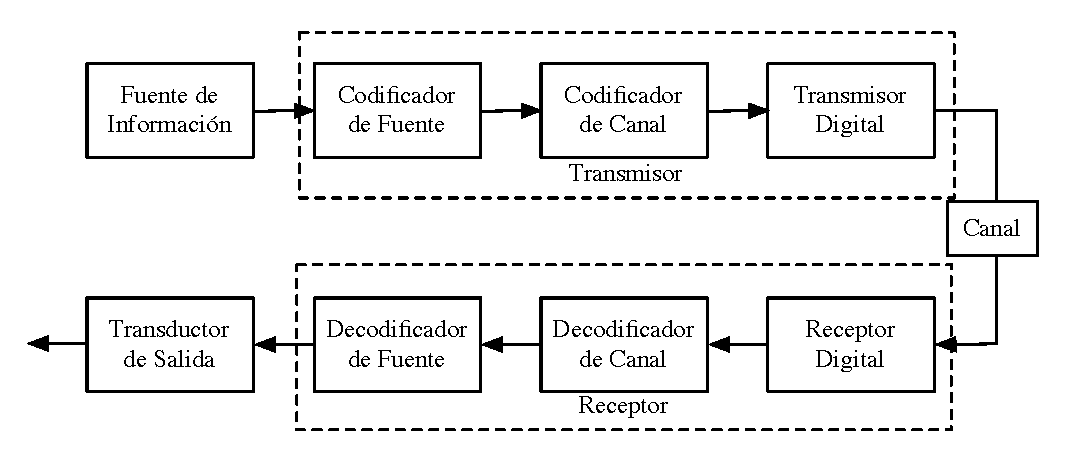
\includegraphics[width=0.95\linewidth]
{introduccion/figuras/fig01-01.pdf}
\caption{Modelo de un sistema de Comunicación Digital I}
\label{fig01-01}
\end{figure}
\end{lstlisting}
%\end{micuadro}

Y el resultado se muestra en la \autoref{fig01-01}.

%
\begin{figure}[htbp]
\centering
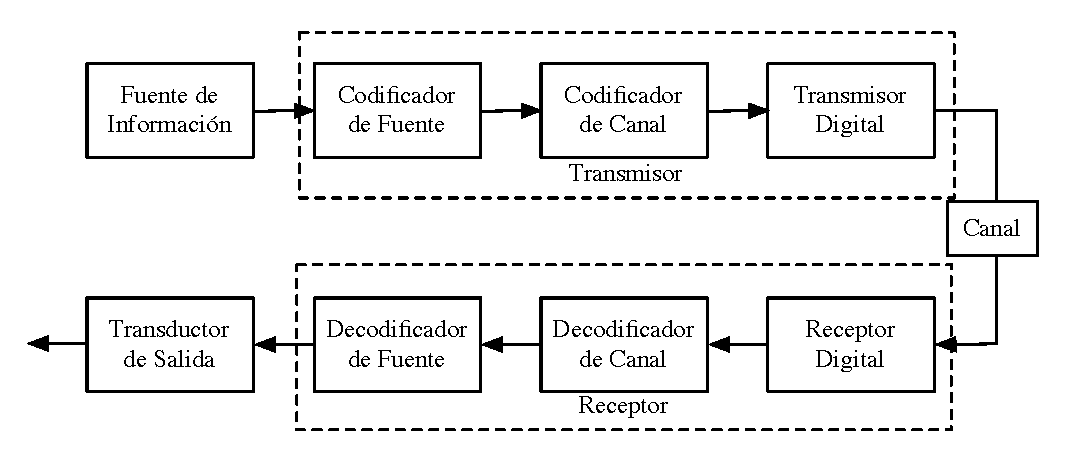
\includegraphics[width=0.95\linewidth]{introduccion/figuras/fig01-01.pdf}
\caption{Modelo de un sistema de Comunicación Digital I}
\label{fig01-01}
\end{figure}
%

Para incluir una tabla utilizamos las instrucciones siguientes:
%\nopagebreak 
\begin{lstlisting}[language=,caption={Inclusión de una tabla}, breaklines=true, label=prg01-02]
\begin{table}[htbp]
	\ttabbox
	{\caption{Tipos de transmisión y frecuencia central} 
	\label{tab2_1}}
		{
		\begin{tabular}{c c}
		\hline
		\rule[-8pt]{0pt}{22pt}{\bfseries{Tipo de Transmisión}}&
		 {\bfseries{Frecuencia central de transmisión}} \\
		\hline
		\rule{0pt}{14pt}Modem & 100-1800 Hz \\
		Radio AM & 530-1600 kHz \\
		Radio FM & 88-108 MHz \\
		Televisión & 178-216 MHz \\
		Telefonía móvil & 850 MHz-1,8 GHz \\
		Redes inalámbricas &  $2,4$ GHz \\
		Fibra óptica & $2\cdot 10^{14}$ Hz \\
		\hline
		\end{tabular}
		}
\end{table}
\end{lstlisting}

Y el resultado se muestra en la \autoref{tab2-1}.

\begin{table}[htbp]
	\ttabbox
	{\caption{Tipos de transmisión y frecuencia central} \label{tab2-1}}
		{
		\begin{tabular}{c c}
		\hline
		\rule[-8pt]{0pt}{22pt}{\bfseries{Tipo de Transmisión}}& {\bfseries{Frecuencia central de transmisión}} \\
		\hline
		\rule{0pt}{14pt}Modem & 100-1800 Hz \\
		Radio AM & 530-1600 kHz \\
		Radio FM & 88-108 MHz \\
		Televisión & 178-216 MHz \\
		Telefonía móvil & 850 MHz-$1,8$ GHz \\
		Redes inalámbricas &  $2,4$ GHz \\
		Fibra óptica & $2\cdot 10^{14}$ Hz \\
		\hline
		\end{tabular}
		}
\end{table}

Observemos  que en la parte inferior de las figuras y en la superior de las tablas (esta ha sido nuestra elección), se colocan textos explicativos sobre las mismas. El formato de este texto se logra mediante una sentencia facilitada por el paquete que se carga mediante el comando \comandos{usepackage}{caption}. El resto de paquetes utilizados realizan diversas tareas como, por ejemplo, \comandos{usepackage}{longtable}, que permite que una tabla se extienda a través de más de una página.

\subsection{Hiperenlaces}
Un primer paso a la hora de crear un documento es generar una versión en formato electrónico del mismo. Hemos decidido que ese formato sea \ttcolor{pdf} . En un formato pdf existe la posibilidad de crear hiperenlaces que facilitan la navegación a lo largo del mismo. Por ejemplo, el índice en un libro en formato pdf se generará, con la propuesta que hemos realizado, creando enlaces a las diversas partes del mismo. O bien, cuando nos referimos a una figura o tabla, es muy útil la existencia de esos enlaces al lugar exacto en el que se encuentra la figura o tabla.  El paquete responsable de realizar todas estas tareas se denomina \ttcolor{hyperref} y las sentencias que siguen a su carga realizan diversas tareas que pueden consultarse en la extensa documentación que lo acompaña. Sobre la línea 110 de \ttcolor{libroTipoETSI.tex} encontrará que puede modificar el color del enlace, puesto a negro por defecto.
% Por ejemplo, no habrá que olvidarse sustituir el literal \ttcolor{F. Javier Payán Somet y Juan José Murillo Fuentes} por el nombre del autor correspondiente.

\subsection{Tabla de contenido}
La generación de la tabla (o tablas) de contenido de un texto suficientemente largo suele ser una tarea sumamente laboriosa. \LaTeX\ facilita enormemente este trabajo mediante un conjunto de paquetes y comandos que se agrupan bajo el apartado genérico denominado TOC (Table Of Contents). En otra sección de este capítulo explicaremos cómo y dónde se incorporará esta tabla de contenidos. En este apartado nos centramos en explicar algunos aspectos de cómo se construye la principal tabla de contenidos, que denominamos  \ttcolor{Índice}.

Nuestra primera decisión fue establecer que en el índice deben aparecer hasta los apartados que hemos denominados \ttcolor{subsubsecciones}, lo que se logra mediante el \ttcolor{\{3\}} del comando \comandos{setcounter}{tocdepth} en \ttcolor{libroETSI.sty}. El formato de cada uno de los apartados se logra con el conjunto de sentencias que siguen y tienen una estructura bastante autoexplicativa. También hemos propuesto que no aparezcan los habituales puntos que existen entre el texto y el número de página correspondiente de muchos índices, ajustando a \ttcolor{10000} el parámetro \ttcolor{\textbackslash@dotsep}. 

Nuestra siguiente decisión afecta a la manera en la que hemos querido que aparezcan en el índice los índices del texto, valga la redundancia. No es trivial pero, básicamente, hemos definido dos listas, una para los elementos que aparecen antes del Índice General y otra para los  que aparecen después, al fina del texto, que se corresponden aproximadamente a lo que hemos denominado \ttcolorc{frontmatter} y \ttcolorc{backmatter}, respectivamente. Si no se desea cualquier índice, basta con comentar la línea correspondiente.

\subsection{Formatos de títulos, páginas y cabeceras y pies de páginas}
El aspecto de un libro está básicamente definido por el formato que se ha elegido para los diferentes títulos de las partes que lo constituyen, el formato de las páginas y qué queremos que aparezca en las cabeceras y pies de páginas del mismo. Todo esto se ha conseguido utilizando un paquete desarrollado por el español Bezos denominado \ttcolor{titlesec}, que se carga en nuestro fichero mediante la instrucción \comandos{usepackage[noindentafter, pagestyles,...]}{titlesec}.

El paquete nos permite definir los distintos tipos de páginas, de acuerdo con las instrucciones que se proporcionan en el mismo. Por ejemplo, con \comandos{newpagestyle}{esitscCD} creamos la página habitual en la mayor parte del texto, formada por el número en la parte exterior de la misma, en las páginas pares el nombre del capítulo en el que estamos y en las impares el nombre de la sección. Estos elementos se colocan encima de una raya horizontal que se ha definido previamente, tanto en su grosor como en su longitud.

Una vez definidos las diferentes tipos de páginas podemos definir, por ejemplo, que nuestra página por defecto será \ttcolor{esitscCD}, con la instrucción \comandos{pagestyle}{esitscCD}. Si queremos que una página determinada en un punto concreto sea diferente, si suponemos que, por ejemplo, el estilo de página \ttcolor{otroestilo} ha sido definido, basta situar la instrucción \comandos{thispagestyle}{otroestilo} en el punto deseado. Un ejemplo podemos encontrarlo en la manera que logramos que los capítulos empiecen siempre en páginas impares. Con ese fin, se utiliza el estilo de página \ttcolor{empty} en caso de que sea necesario.

Por último, el paquete \ttcolor{titlesec} nos permite definir cómo queremos que sean los titulares que usaremos en nuestros textos. Así,  la instrucción \comandos{titleformat}{\textbackslash section ...} establece que nuestras secciones estarán numeradas al nivel de capítulo, con el número de la sección fuera de margen \ttcolor{hang}, y con unas determinadas separaciones del texto, establecidas a través del comando \ttcolorc{titlespacing}. 

En todo caso, estos parámetros no se deberían de tocar, salvo en contadas ocasiones, y por ello se incluyen aquí estos detalles.

\subsection{Teoremas, propiedades, definiciones y demás}
En la escritura de cualquier texto científico los Teoremas, propiedades y demás elementos constituyen una parte muy significativa. Existen, de nuevo, múltiples posibilidades de tratar estos elementos, pero hemos considerado que las facilidades que suministra el paquete \ttcolor{ntheorem}, cargado mediante la instrucción \comandos{usepackage [thmmarks, amsmath, noconfig, hyperref, framed]}{ntheorem} se adapta perfectamente a nuestros gustos y decisiones. Por ejemplo, con el conjunto de instrucciones que se muestran en  el Código \ref{prg01-03}:

\begin{lstlisting}[language=TeX,caption={Teoremas, Lemas,...}, breaklines=true, label=prg01-03]
\theoremnumbering{arabic}
\theoremheaderfont{\aheadteoremas}
\theoremseparator{\hspace{.2em}}
\theorembodyfont{\itshape}
\newtheorem{teor}{Teorema}[section]
\newtheorem{lema}{Lema}[section]
\newtheorem{prop}{Propiedad}[section]
\newtheorem{coro}{Corolario}[teor]
\end{lstlisting}

\noindent hemos definido los Teoremas, Lemas, Propiedades y Corolarios. Centrándonos en los teoremas, las instrucciones anteriores definen que los teoremas estarán referenciados mediante un número \ttcolor{arabic}, con una numeración que será creciente desde la unidad dentro de cada sección de un determinado capítulo, \comandos{newtheorem\{teor\}}{Teorema}\ttcolor{[section]}. La fuente que se utilizará para que aparezca la palabra ``Teorema'' está definida por el comando \ttcolor{\textbackslash theoremheaderfont\{\textbackslash aheadteoremas\}}, el enunciado del teorema se realizará en itálica y para enunciar un teorema y su demostración utilizamos las siguiente instrucciones:

\begin{lstlisting}[language=TeX,caption={Teorema y Demostración}, breaklines=true, label=prg01-04]
\begin{teor}[Teorema de Pitágoras]
En un triángulo rectángulo...
\end{teor}
\begin{proof}
Sea el triángulo ABC...
\end{proof}
\end{lstlisting}

El resultado sería el siguiente:
\begin{teor}[Teorema de Pitágoras]
En un triángulo rectángulo...
\end{teor}
\begin{proof}
Sea el triángulo ABC...
\end{proof}

Podemos observar que al finalizar la demostración hemos incluido el símbolo $\blacksquare$. De manera análoga, están definidas las restantes entidades, incluyendo el comando que nos permite escribir los cuadros de elementos de la programación.

\subsection{Índices de palabras y glosarios}
Con los paquetes index y glossaries podemos incluir índices de palabras y listas con definiciones, ya sea de acrónimos u de otro tipo. Por ejemplo, se podría usar también para definir magnitudes o la notación utilizada.
 
%http://en.wikibooks.org/wiki/LaTeX/Indexing
\subsubsection{Índices de palabras}
\index{Indice de palabras@Índice de palabras!index}%\index{\'Indice de palabras!index}\index{Índice de palabras!indexit}
Para construir un índice de palabras\index{Indice de palabras@Índice de palabras}, como el que puede encontrar al final de este texto, se incluye el paquete \comandos{usepackage}{imakeidx} con algunas opciones. Para incluir una palabra  en el índice utilizamos   \comandos{index}{palabra} justo detrás de la palabra que queramos indexar. Si queremos agrupar en un grupo diferentes subpalabras \index{Indice de palabras@Índice de palabras!subpalabra}, utilizamos \comandos{index}{palabra!subpalabra}. Es importante no olvidar ejecutar \ttcolor{makeindex}, al igual que ejecuta latex o bibtex para componer el texto o generar la bibliografía. Otro detalle importante es poner los índices con mayúsculas o con minúsculas, pero todos iguales. De esta forma, cuando se genere el índice de palabras no queden algunas con la primera letra en mayúsculas y otras no. Por último, con las instrucciones de compilación que se detallan un poco más adelante, las palabras en español que empiecen por tilde se indexan al final. Para evitarlo, y que aparezcan en su sitio, tiene que escribir primero la palabra sin tilde seguida de arroba y la palabra con tilde, como por ejemplo \ttcolorc{index\{Indice de palabras@Índice de palabras\}}. 

\subsubsection{Glosario}
Un glosario con acrónimos u otros términos se realiza en este texto utilizando\\
 \comandos{usepackage [acronym]}{ glossaries}. 
 Para definir un acrónimo, basta con incluir antes del comienzo del documento una línea del tipo:\\
 \comandos{newacronym[type=main]\{etiqueta\}\{acrónimo\}}{nombre completo}, 
 \\
 como por ejemplo\\
 \comandos{newacronym[type=main]\{ETSI\}\{ETSI\}}{Escuela Técnica Superior de \\Ingeniería}. 
 \\
 En esta orden el primer argumento es el identificador o etiqueta, el segundo es el acrónimo o abreviatura y el tercero es el nombre completo al que hace referencia el acrónimo o abreviatura. Para utilizar luego la abreviatura o acrónimo, y se pueda luego generar un índice que indique en qué página se ha usado, se utiliza \comandos{gls}{etiqueta}. 

\subsubsection{Compilación de índices de palabras y glosarios}
Existen distintos comandos para generar el índice y el glosario. Puede utilizar los que estime oportunos. Aquí se ofrece una solución para realizarlo.

El comando más usado es \ttcolor{makeindex}. Habría que llamar dos veces a este comando, con distintos argumentos, si se incluye el glosario además del índice. En Macintosh si utiliza el comando \ttcolor{lualatexmk}, uno de los engines de TeXShop\index{engine}, el índice de palabra y el glosario se generarán de forma automática. 
%Puede usar Texindy\index{Texindy} para una presentación del índice de palabras con otra presentación.

En Windows, tendrá que ejecutar PDFLatTeX ó LatexMk, luego tendrá que ejecutar makeindex tal cual para generar el índice de palabras. Para generar el glosario tendrá que definir un comando de usuario, tal como sigue. Vaya al menú `Usuario', en texmaker, y allí a `Comandos de Usuario' y dentro de este a `Editar Comandos de Usuario'. En cualquiera de los comandos defina uno nuevo con el título que quiera, por ejemplo glosario, y en el campo comando, incluya la siguiente línea\footnote{Si usase el texmaker en Mac-OS tendría que pulsar el asistente para seleccionar makeindex. Aparecería en el campo comando algo así como \ttcolor{''makeindex'' \%.idx}, donde el asistente habrá encontrado la carpeta donde está el comando makeindex. Sustituya el final, \%idx, por  -s \%.ist -t \%.glg -o \%.gls \%.glo, de forma que el campo comando quede como sigue:
 \ttcolor{''/usr/texbin/makeindex'' -s \%.ist -t \%.glg -o \%.gls \%.glo}}

Una vez definido este comando de usuario, ejecútelo, y vuelva a ejecutar PDFLaTeX o LatexMk.

\section{Antes del documento}
Antes de empezar la edición del documento, además de cargar los ficheros de estilos \ttcolor{LibroETSI.sty} y \ttcolor{edicionLibro.sty} (o el correspondiente al documento),  hemos creído necesario realizar una serie de operaciones que faciliten nuestro trabajo o lo configuren de una determinada manera. %Además, hay que incluir la portada.

\subsection{Fichero de notación: notacion.sty}
Hemos considerado interesante incluir un fichero de notaciones que son de amplia utilidad dentro del área de conocimiento de los autores. Su uso es completamente opcional pero se ha utilizado ampliamente en la elaboración de este texto. Simplifica enormemente la escritura hacer uso de ficheros de este tipo y prácticamente cada autor utiliza el suyo propio.

Como ocurría con el fichero \ttcolor{LibroETSI.sty}, es necesario que se cargue, incluyendo la instrucción \comandos{usepackage}{notacion} al comienzo del fichero principal. Puesto que su uso resulta evidente, no hemos considerado necesario realizar una documentación precisa sobre el mismo más allá de los propios comentarios que acompañan las definiciones del fichero, y que el lector puede consultar abriéndolo. Nótese que existe además una carpeta con este nombre. En esta carpeta se ha incluido un ejemplo de notación que podría ponerse al comienzo de un documento. Sobre este documento, se puede añadir o quitar lo que se desee.

\subsection{Fuente del texto}
Las instrucciones incluidas en el código \ref{prg01-05} y que pertenecen al fichero \ttcolor{LibroETSI.sty} 
 se pueden modificar para cambiar la fuente del texto.  En primer lugar, debemos actuar de forma diferente si queremos utilizar la fuente Minion Pro o no.  Si hemos definido como \ttcolor{true} el parámetro correspondiente, en el caso que estemos compilando con \LaTeX\ no debemos hacer nada. Sin embargo, en el caso de utilizar \LuaLaTeX\ debemos declarar que la fuente va a ser Minion Pro y modificar ligeramente su tamaño.
 
Si no vamos a utilizar una fuente Minion Pro, en el caso de \LuaLaTeX\ se puede utilizar para el texto cualquier fuente OTF o TTF que el usuario posea de forma legal, y se encuentre instalada, lo que depende del sistema operativo (SO) utilizado. En nuestro caso, observad que hemos utilizado una fuente Time New Roman  pues suele estar instalada en la mayoría de los SO. Se proponen asimismo un par de alternativas si prefiere otras fuentes.
 
El código incluido detecta si se no se está utilizando \LuaLaTeX\, en cuyo caso se usa una fuente equivalente a una Times, cargada mediante el comando estándar \comandos{usepackage}{tgtermes}. Hay otras opciones comentadas, y se pueden buscar otras fuentes. 
 
\begin{lstlisting}[language=,caption={Fuente del texto}, breaklines=true, label=prg01-05]
%:Para modificar fácilmente la fuente del texto. 
\makeatletter
\ifdtsc@Minion % Queremos utilizar la fuente Minion y lo hemos declarado al principio
	\ifluatex
		\setmainfont[Renderer=Basic, Ligatures=TeX,	% Fuente del texto 
		Scale=1.01,
		]{Minion Pro}
   		% En este caso conviene modificar ligeramente el tamaño de las fuentes matemáticas
		\DeclareMathSizes{10}{10.5}{7.35}{5.25}
		\DeclareMathSizes{10.95}{11.55}{8.08}{5.77}
		\DeclareMathSizes{12}{12.6}{8.82}{6.3}
	\fi
\else
	\ifluatex
		% Para utilizar la fuente Times New Roman, o alguna otra que se tenga instalada
		\setmainfont[Renderer=Basic, Ligatures=TeX,	% Fuente del texto 
		Scale=1.0,
		]{Times New Roman}
%		\setmainfont[Renderer=Basic, Ligatures=TeX,	% Fuente del texto 
%		]{Adobe Garamond Pro}
%		\setmainfont[Renderer=Basic, Ligatures=TeX,	% Fuente del texto 
%		]{Palatino LT Std}
	\else
		\usepackage{tgtermes} 	%clone of Times
		%\usepackage[default]{droidserif}
		%\usepackage{anttor} 	
	\fi
\fi
\makeatother
\end{lstlisting}

Si se intenta utilizar una fuente que no está instalada (dentro del sistema operativo) la compilación con \LuaLaTeX\ daría error. Si se instala una nueva fuente y se desea utilizar, se puede tratar de modificar las líneas de código que se suministran como ejemplo. La primera vez que se utilice esa nueva fuente, \LuaLaTeX\ tardará algo más en compilar pues necesita generar una serie de ficheros internos.

La principal ventaja en el uso de \LuaLaTeX\ la encontramos en la facilidad para utilizar diferentes fuentes en diferentes lugares y con diferentes características (tamaño, color, etc) muy fácilmente configurables. Puede ser interesante leer el fichero \ttcolor{fontspec.pdf} para conocer cómo se realizan estos cambios. 

En caso de utilizar el motor pdfLatex, la elección más sencilla se realiza como hemos dicho mediante paquetes específicos tales como \comandos{usepackage}{tgtermes}. Puede consultarse la dirección \url{http://www.tug.dk/FontCatalogue/alphfonts.html} para conocer las posibilidades más habituales. 

Por último: como ya hemos dicho, todo lo anterior únicamente afecta a la elección de las fuentes del texto. La elección de las fuentes matemáticas (texto dentro de matemática, símbolos, letras griegas, etc) se controla de manera completamente diferente mediante paquetes específicos. En el \autoref{estilo} volveremos sobre este asunto. En concreto, observar que en el caso de compilar con la opción \ttcolor{Minion=true} y existir el fichero de estilo \ttcolor{MinionPro.sty} (no confundir con la fuente Minion Pro; si no existiera el fichero, aparecería un error), se propone el uso de la fuente Minion Pro como fuente matemática, junto con los símbolos de la fuente MnSymbol. En caso contrario, se hará uso de una fuente Times (en realidad, de una extensión de la misma). 

No todas las fuentes pueden usarse como fuentes matemáticas y en la dirección \url{http://www.tug.dk/FontCatalogue/alphfonts.html} se encuentran recogidas las que si tienen soporte matemático. Es importante señalar además que no todas las combinaciones de fuente de texto y fuente matemática son tipográficamente adecuadas. 

\subsection{Cubierta y primeras páginas}
Se ha diseñado esta plantilla para que tome una imagen de fondo y a partir de ésta se incluyan los datos de título, autor, etc, para generar la portada del documento. La portada propuesta es distinta para proyectos fin de carrera y similares que para libros o tesis. Todo esto se ha hecho diseñando una serie de funciones que las generan, tomando los datos que se definen en la cabecera del fichero principal. Así, en el \ttcolor{libroTipoETSI.tex}, se puede definir el título de la obra, el autor, etc. En el caso de \ttcolor{pfcTipoETSI.tex} y \ttcolor{tesisTipoETSI.tex}, se puede definir además el director, el tipo de proyecto (máster, grado y carrera), y otros parámetros. Las imágenes de fondo de la cubierta también se llaman desde este fichero, así como la imagen al pié de la hoja interior con el título y autor de la obra (para libros). La imagen central de la cubierta está en la carpeta figuras, con nombre \ttcolor{imagenLibro.png}. Puede incluir la imagen deseada en esta carpeta salvándola con este mismo nombre. Preste atención a que el formato es rectangular. Para introducir la imagen del logo del departamento en el proyecto fin de carrera/grado/máster, puede retocar la imagen de fondo, cortando el logo existente e insertando el deseado. Estas imágenes están en la carpeta figuras. 

Para cambiar cualquier otro aspecto, tales como el tamaño de la figura de la cubierta ó los créditos de la cubierta, tendrá que modificar el fichero \ttcolor{edicionLibro.sty} en este caso de un libro. 

%En el ejemplo que se presenta para libros, el latex toma una imagen de fondo, y otra, imagenLibro.png,  de la portada para incluir además de los datos de título y autores, definidos al comienzo del fichero \ttcolor{portadaLibro.tex}, una imagen superpuesta representativa de la temática del texto. Los autores pueden cambiar esta imagen fácilmente por otra acorde a su texto.

%Sería interesante poner algo sobre citas

\endinput
%Guia uso


%% !TEX root =../LibroTipoETSI.tex
%El anterior comando permite compilar este documento llamando al documento raíz
\chapter{Notas sobre la Redacción del Texto}\label{chp-01}
\epigraph{Texto elaborado por Marísa Balsa, de la Biblioteca de la Escuela Técnica Superior de Ingeniería de la Universidad de Sevilla}%{Claude Shannon, 1948}

%\lettrine[lraise=0.7, lines=1, loversize=-0.25]{E}{n}
\lettrine[lraise=-0.1, lines=2, loversize=0.2]{S}{e} recomienda consultar la norma UNE 50136:1997: Documentación, presentación de tesis y documentos similares. Por otro lado, existen recursos en línea que ayudan a organizar todo el proceso de elaboración del Trabajo. El personal de la Biblioteca imparte formación y asesoramiento sobre su uso.  
Para establecer la estructura y orden de los datos y partes del Trabajo Fin de Grado nos basamos en la Normativa de los Trabajos Fin de Grado de la Escuela Técnica Superior de Ingeniería de Sevilla (Aprobada en la sesión de la Junta de Escuela de 12 de julio de 2013, modificada en Junta de Escuela de 05 de febrero de 2014) y en la norma UNE 50136:1997: Documentación, presentación de tesis y documentos similares.

\section{Preliminares}
\subsection{Cubierta}
Deberá utilizarse la plantilla aprobada por la Junta de Escuela del 25/4/2014 que se describe en este texto y cuyo modelo puede tomarse de este documento. Debe contener todos los datos que se especifican y en el orden y modelo que se establece: nombre completo del autor, título del Trabajo, nombre completo del tutor, nombre del Departamento, fecha, Grado al que se opta, etc.
\subsection{Portada}
Igulamente deberá utilizarse la plantilla… y contener todos los datos que figuran en ésta, en el orden especificado: el nombre de la Escuela, la titulación y, en su caso, la intensificación, el título del TFG, los nombres del autor, del tutor(es) y, en su caso, del ponente, el Área de Conocimiento, el Departamento y el año de ejecución del proyecto.
\subsection{Resumen} 
Texto que muestra de forma abreviada y precisa el contenido del trabajo. Se podrá también incorporar una versión en inglés que se colocará a continuación precedida del término Abstract.
\subsection{Prefacio o Introducción}
Debe incluir una breve explicación de las razones que han llevado a la realización del Trabajo, el propósito y los objetivos que se pretenden, el ámbito, alcance y límites de la investigación, así como la metodología empleada y, si se considera oportuno, un avance de las conclusiones alcanzadas.  

\subsection{Índice y/o Índice general}
Tabla de contenidos donde se reflejan todas las partes del Trabajo y sus anexos, si los hubiera. Deben aparecer los títulos, en su orden y con indicación de la página en la que se pueden encontrar.
Si el Trabajo consta de varios volúmenes, cada uno deberá llevar su propio índice, pero se debe incluir también un índice general.
\subsection{Lista de ilustraciones y tablas}
Si el Trabajo incluye ilustraciones y tablas se puede añadir un listado que incluya el número identificativo que figura dentro del texto, la leyenda y el número de la página en la que se encuentra.
También es conveniente mencionar los datos sobre las fuentes de donde se han obtenido dichas ilustraciones si no se han incluido en el propio texto de la memoria.
\subsection{Lista de abreviaturas y símbolos}
El Trabajo debe contener las abreviaturas y símbolos internacionalmente reconocidos. Si se incorporan unidades, abreviaturas o acrónimos que puedan ser poco conocidos se deberán explicar brevemente en estas listas.
\subsection{Glosario}
Los términos que requieran definición o explicación se deberán incorporar en un glosario.
\section{Texto principal}
Para su elaboración es importante tener en cuenta su distribución en capítulos y secciones numeradas, siguiendo la plantilla elaborada por…. 
El texto debe comenzar con una introducción que muestre las investigaciones previas existentes sobre el tema y destacar los objetivos y métodos seguidos para llevar a cabo la investigación o análisis del tema tratado.
Para finalizar se deben escribir las conclusiones que deben estar en relación con los objetivos marcados previamente.
\section{Bibliografía}
Debe contener las referencias bibliográficas de los documentos consultados para demostrar las bases del trabajo realizado y avalar los datos incorporados y citados en el texto.
Se elaborará de forma normalizada, para lo que se aconseja utilizar la norma UNE vigente (actualmente la “UNE ISO 690:2013. Información y documentación. Directrices para la redacción de referencias bibliográficas y de citas de recursos de información”).
Para la elaboración de esta parte del Trabajo se recomienda consultar la Web de la Biblioteca de Ingeniería que contiene recursos, guías y ayudas para la elaboración de las referencias bibliográficas. 
\section{Anexos}
Se puede incluir de esta forma material extenso utilizado en el trabajo, importante para justificar los resultados y las conclusiones obtenidas, pero que no es esencial para la comprensión del texto principal. Pueden ser datos estadísticos, legislación, etc.
La paginación debe ser correlativa y continuar la del texto principal. Cada uno de los anexos debe identificarse con una letra mayúscula del alfabeto, comenzando por la letra A, precedida de la palabra Anexo

\endinput


% !TEX root =../LibroTipoETSI.tex
\chapter{Ejemplo de Capítulo}\LABCHAP{CAPEJ}
\pagestyle{esitscCD}
\epigraph{ Una de las virtudes del ingeniero es la eficiencia.  }{Guang Tse}

%\lettrine[lraise=0.7, lines=1, loversize=-0.25]{E}{l} 
\lettrine[lraise=-0.1, lines=2, loversize=0.25]{E}l \emph{formato de capítulo }\index{formato!de capítulo} abarca diversos factores. Un capítulo puede incluir, además de texto, los siguientes elementos:
%http://en.wikibooks.org/wiki/LaTeX/List_Structures#Customizing_Lists

\begin{itemize}\itemsep1pt \parskip0pt \parsep0pt
\item \indexit{Figuras}
\item \indexit{Tablas}
\item \indexit{Ecuaciones}
\item \indexit{Ejemplos}
\item \indexit{Resúmenes}, con recuadros en gris, por ejemplo
\item \indexit{Lemas}, \indexit{corolarios}, \indexit{teoremas},... y sus demostraciones
\item \indexit{Cuestiones}
\item \indexit{Problemas} propuestos
\item ...
\end{itemize}

En este capítulo se propone incluir ejemplos de todos estos elementos, para que el usuario pueda modificarlos fácilmente para su uso. Consulte el código suministrado, para ver cómo se escriben en \LaTeX.

\section{Ejemplo de sección}\LABSEC{SEC}
%
En la \FIG{FIG} se incluye a modo de ejemplo la imagen del logo de la \gls{ETSI} \footnote{Se usa aquí el package de acrónimos, que la primera vez define el acrónimo y ya luego sólo incluye el mismo. Esto facilita luego generar de forma automática la lista de acrónimos.}. El código para que aparezca dicha imagen se muestra en el cuadro siguiente:



Si nos detenemos en los comandos que hemos utilizado, con \ttcolor{width} se controla el ancho, y se escala así el tamaño de la imagen. En \LaTeX existen diversas opciones para situar la figura en la página: con \ttcolor{t} o \ttcolor{b} se le indica que las incluya arriba o abajo (top/bottom) y con \ttcolor{!} se le pide que la deje dónde está, tras el texto anterior.


\begin{lstlisting}[language=TeX,caption={Código para incluir una figura}, breaklines=true, label=prg01-01]
\begin{figure}[htbp]
\centering

\includegraphics[width=3 cm]{capituloLibroETSI/figuras/logoESI.pdf}
\caption{Logo de la ETSI}
\label{fig:figura1}
\end{figure}
\end{lstlisting}


\begin{figure}[htbp]
\centering
%
\includegraphics[width=0.2\linewidth]{capituloLibroETSI/figuras/logoESI.pdf}

\includegraphics[width=3 cm]{capituloLibroETSI/figuras/logoESI.pdf}
\caption{Logo de la ETSI}
\LABFIG{FIG} %Esto es una forma propia de los autores de gestionar las etiquetas y referencias
\end{figure}
%

Para dar énfasis a algún texto, usamos \ttcolorc{emph}. %Este comando es de los denominados \emph{inteligentes} apareciendo el texto \emph{resaltado} dependiendo del contexto.  
Así, por ejemplo, 
\begin{caja}
\emph{No olvide intentar utilizar este formato en sus publicaciones de la \gls{ETSI}}
\end{caja}
hace aparecer el anterior texto en itálica. Pero si escribiésemos, por ejemplo, 
\begin{caja}
\emph{No olvide intentar utilizar este formato \emph{siempre} en sus publicaciones de la \gls{ETSI}}
\end{caja}
vemos cómo hemos destacado la palabra ``siempre'' en torno a su contexto. Para ello, hemos escrito, realmente, \comandos{emph}{siempre} dentro de la frase original.
%
\subsection{Ejemplo de subsección}\LABSSEC{EjSS}
%
Si se usaba \ttcolorc{section} para indicar una sección, se utiliza \ttcolorc{subsection} para una subsección.


\section{Elementos del texto}
%

\subsection{Figuras}

Además del tipo de figura que vimos anteriormente, el normal, podemos desear incluir una figura en modo apaisado ocupando toda la página. Para ello utilizamos el entorno de figura siguiente \comandos{begin}{sidewaysfigure}, cuyo resultado se puede observar en la \FIG{FigApaisada}. 

\begin{sidewaysfigure}
\centering
%
\includegraphics[width=0.2\linewidth]{capituloLibroETSI/figuras/logoESI.pdf}

\includegraphics[width=3 cm]{capituloLibroETSI/figuras/logoESI.pdf}
\caption{Logo de la ETSI}
\LABFIG{FigApaisada}
\end{sidewaysfigure}

Aunque puede optar por la forma que desee, en el fichero \ttcolor{notacion.sty} se incluyen definiciones para que pueda usar \comandos{LABFIG}{etiqueta} y \comandos{FIG}{etiqueta} para poner una etiqueta y hacer referencia a la misma luego. Además, está definido para que \comandos{FIG}{etiqueta} incluya por delante el término Figura.

\subsection{Tablas}
A modo de ejemplo, \TAB{Tab1} incluye un ejemplo de tabla. Al igual que con figura, si usa \ttcolor{notacion.sty} puede usar \comandos{LABTAB}{etiqueta} y \comandos{TAB}{etiqueta} para poner una etiqueta y una referencia, y el \comandos{TAB}{etiqueta} ya incluye el nombre Tabla por delante.

Una alternativa al uso de estos comandos está representado por el uso del comando \ttcolorc{autoref\{etiqueta\}} que, en conjunción con el paquete \ttcolor{babel} genera automáticamente los nombres de Figura o Tabla, en función de la etiqueta correspondiente.

\begin{table}[h]
%\small
\caption{Valores de parámetros}
\begin{center}
\begin{tabular}{p{7cm}p{2cm}p{2cm}} %Con esto definimos el ancho de cada columna
Definición & notación & valor\\
 \hline
Potencia transmitida	(entregada a antena) & $P_{et}$ & -5 a 20 dBm	\\
Ganancia antenas & $G$ & $40.5$ dBi\\	
 \hline
\end{tabular}
\end{center}
\LABTAB{Tab1}
\end{table}%

\subsection{Listados de programas}
Es muy habitual en nuestros documentos que tengamos que incluir listados de programas. Para ello, se propone la utilización de un paquete denominado \ttcolor{listings}. Se obtiene con él un listado como el mostrado en el \autoref{prg02-01} de \matlab siguiente: 

\begin{lstlisting}[language=Matlab,caption={Representación de la función $\rect(t-T/2)$}, breaklines=true, label=prg02-01]
clear all
close all
T = 1;
A = 1;
L = 100;
tstep = T/L;                                
t = 0:tstep:T-tstep;   
g_t = A*ones(1,L); 
figure(1);
subplot(211);
h=plot(t,g_t); axis( [0 T -A-0.1 A+0.1]);
set(h,'linewidth', 1.0);
ylabel('g(t)'), xlabel('t[s]'); grid on;

g_n = g_t;
subplot(212);
h=stem(g_n, '.', 'filled'); axis( [1 L -0.1 A+0.1]);
set(h,'linewidth', 1.0);
ylabel('g(n)'), xlabel('n');
\end{lstlisting}

También se puede generar en este caso una relación de los códigos usados en nuestro documento, de manera equivalente a la relación de figuras o tablas. Para ello, observar la correspondiente codificación en el fichero principal.
 
\subsection{Ecuaciones}%%%%%%%%%%%%%%%%%%%%%%%%%%%%%%%%%%%%%%%
Para escribir expresiones matemáticas, como por ejemplo $2+2=4$, sólo hace falta que meta la expresión entre símbolos \ttcolor{\$}. En el fichero notacion.sty se incluyen muchas definiciones para facilitar la escritura de estas expresiones y de ecuaciones. Para escribir una ecuación, con una o más líneas, se aconseja utilizar \ttcolor{align}, como en el siguiente ejemplo, en las ecuaciones \EQ{Eq1}-\EQ{Eq3},
\begin{align}
 T     &=kT_b  \LABEQ{Eq1}, \\
 R_b&=\frac{1}{T_b }	, \\
 D    &=\frac{1}{T}=\frac{R_b }{k}=\frac{R_b}{\log_2 M}. \LABEQ{Eq3}
\end{align}
Si no quiere numerar una línea, utilice las instrucción \comando{nonumber} antes de poner \verb+\\+  para escribir la siguiente línea. Y con \& puede alinear las ecuaciones. 

Un ejemplo más complejo de ecuaciones sería el siguiente: decimos que el vector aleatorio $\vc{Z}$ es gaussiano si su función densidad de probabilidad conjunta viene dada por:
\begin{equation}\label{eq02-x131}
f_{\vc{Z}}\left( {\vc{z}} \right)= \frac{1}{\left( {2\pi} \right)^{N}{\left| {\vc{C_{Z}}} \right|}^{1/2}}\e^{-\frac{1}{2}\left( {\vc{z}-\vc{m_{Z}}} \right)\trs\vc{C_{Z}}^{-1}\left( {\vc{z}-\vc{m_{Z}}} \right) }
\end{equation}con el vector media la matriz $\vc{m_{Z}}$ y la matriz de covarianza real $\vc{C_{Z}}$ $\left( {2N \times 2N} \right)$ simétrica definida positiva dado por:
\begin{equation}\label{eq02-x132}
\vc{m_{Z}}=\begin{bmatrix}
\vc{m_{X}}\\
\vc{m_{Y}}
\end{bmatrix}, \quad
\vc{C_{Z}}=\begin{bmatrix}
\vc{C_{X\hphantom{X}}} & \vc{C}_\vc{XY}\\
\vc{C_{YX}} & \vc{C_{Y\hphantom{X}}}
\end{bmatrix}
\end{equation}con el vector $\bm{\omega}$ dado por:
\begin{equation}\label{eq02-y410}
\bm{\omega}=\begin{bmatrix}
\omega_{1}\\
\vdots \\
\omega_{N}\\
\omega_{N+1}\\
\vdots \\
\omega_{2N}
\end{bmatrix}
\end{equation}
Si no desea que se numere una ecuación puede poner asterisco, tanto en el entorno \verb+equation+ como \verb+align+.


\subsection{Ejemplos}%%%%%%%%%%%%%%%%%%%%%%%%%%%%%%%%%%%%%%%

Para incluir un ejemplo, utilize el entorno \comando{ejmp}, usando el entorno \comando{begin\{ejmp\}} y \comando{end\{ejmp\}}, y para la solución el entorno  \comando{begin\{sol\}}. 

\begin{ejmp}
Calcule $2+2$.
\end{ejmp}
\begin{sol}
%
Para resolver esto se puede utilizar que $1+1=2$, de la siguiente forma
\begin{equation*}% con el * se evita que se numere la ecuación
2+2=(1+1)+(1+1)=4,
\end{equation*}
donde se ha contado, pruebe a utilizar los dedos de su mano, a cuatro.
\end{sol}

Observad que antes de comenzar el ejemplo y tras su finalización se han incluido unos \emph{filetes} a modo de resalte en el texto. En el caso de una serie de ejemplos, los entornos \comando{begin\{ejmpn\}} y  \comando{begin\{soln\}}, junto con los entornos de cierre correspondientes, permiten que no existan estos filetes entre los ejemplos y soluciones intermedias de la serie.
 
\subsection{Lemas, teoremas y similares}

Se incluyen ejemplos de estos elementos de texto. Empezamos con la \DFN{D11} y la \PRP{P11}:

\begin{defn}[Suma]\LABDFN{D11}
 La suma es la operación que permite contar sobre un número, otro.
\end{defn}


\begin{prop}[Suma]\LABPRP{P11}
 Los números enteros se pueden sumar.
\end{prop}


\begin{lema}[Suma de 1 y 1]\LABLEM{L11}
 La suma $1+1$ es igual a $2$.
\end{lema}
\begin{proof}
Ponga un dedo a la vista, junto a otro, y cuéntelos.
\end{proof}


\begin{teor}[Suma]\LABTHM{T11}
 La suma de cualquier número y dos es igual a la suma del mismo número más uno más uno.
\end{teor}
\begin{proof}
Por inducción y el \LEM{L11}.
\end{proof}

\begin{coro}[Contables]\LABCOR{C11}
  Los números enteros son contables.
\end{coro}
\begin{proof}
Por el \THM{T11}.
\end{proof}


\subsection{Resúmenes}%%%%%%%%%%%%%%%%%%%%%%%%%%%%%%%%%%%%%%%
Para incluir un resumen de una sección o un conjunto de secciones o en cualquier otro punto que consideremos interesante, se utiliza el entorno \comando{begin\{Resumen\}}, que admite como parámetro opcional un nombre que queramos asignarle al resumen. Por defecto, se denomina ``Resumen''. Observar que se ha modificado la cabecera de las páginas impares. Una vez finalizado el resumen, con el comando \comando{end\{Resumen\}}, se recupera la anterior cabecera automáticamente. Los resúmenes que se deseen incluir aparecen en la tabla de contenidos como una sección sin numeración, con el nombre elegido o el nombre por defecto de Resumen. En el siguiente ejemplo hemos utilizado este parámetro opcional de nombre.

\begin{Resumen}[Resumen de Teoría de Información]
\noindent Debido al considerable número de definiciones, teoremas y propiedades que hemos descrito en los apartados anteriores, vamos a presentar un resumen de los principales resultados, no necesariamente en el mismo orden que el expuesto anteriormente. Supondremos en este resumen que las variables aleatorias $X$,  $Y$ y $Z$ son discretas, definidas en el alfabeto $\calg{X}$, $\calg{Y}$  y  $\calg{Z}$ respectivamente. 

\subsubsection*{Entropía de una variable aleatoria discreta}
Se define la entropía $H\left( {X} \right)$ de una variable aleatoria discreta $X$ , con función masa de probabilidad $p\left( {x} \right)$, en la forma:
\begin{equation*}
H\left( {X} \right)= -\sum_{x\in \calg{X} }{p\left( {x} \right)\log p\left( {x} \right)}=\E\left[ -{\log p\left( {X} \right)} \right]
\end{equation*}
\begin{enumerate}
\item Se cumple:
\begin{equation*}
 0\le H\left( {X} \right) \le \log \card{\calg{X}}
\end{equation*}
 con la igualdad en la izquierda si y sólo si $p\xb{i}=1$ para algún $x_{i} \in \calg{X}$ y con la igualdad a la derecha si y sólo si la variable aleatoria está uniformemente distribuida; esto es, $p\xb{i}=1/\card{\calg{X}} \; \mbox{para todo }i$.
 \item $H\left( {X} \right)=0$ si y sólo si $X$ es determinista.
\item $H\left( {X} \right)=H\left( {p\left( {x} \right)} \right)$ es una función cóncava en $p\left( {x} \right)$.
\item Se define la \emph{Función de Entropía Binaria} en la forma:
\begin{equation*}
h_{b}\left( {p} \right) \eqdef -p\log p-\left( {1-p} \right)\log\left( {1-p} \right)\end{equation*}
\item La función entropía binaria $h_{b}\left( {p} \right)$ es una función cóncava en $p$.
\item Si $X$ y $\hat X$ son dos variables aleatorias estadísticamente independientes igualmente distribuidas, 
\begin{equation*}
\Pr\left( {X=\hat X} \right) \ge 2^{-H\left( {X} \right)}
\end{equation*}
con la igualdad si y sólo si $X$ tiene una distribución uniforme.
\end{enumerate}

\subsubsection*{Entropía conjunta y entropía condicional}
Definimos la \emph{entropía conjunta} de las variables aleatorias $X$ e $Y$, $H\left( {X,Y} \right)$ en la forma:
\begin{equation*}
H\left( {X,Y} \right)=\sum_{x\in \calg{X} }{\sum_{y\in \calg{Y}}{p\left( {x,y} \right)\log \frac{1}{p\left( {x,y} \right)}}}=\E\left[ {-\log p\left( {X,Y} \right)} \right]
\end{equation*}

Definimos la \emph{entropía condicional} $H\left( {X \mid Y} \right)$ en la forma:
\begin{align*}
H\left( {X \mid Y} \right)&=\sum_{y\in \calg{Y}}{p\left( {y} \right)H\left( {X \mid Y= y} \right)}=  \\
&=-\sum_{x\in \calg{X}}{\sum_{y\in \calg{Y}}{p\left( {x,y} \right) \log p\left( {x \mid  y} \right)}}= \\
&=\E\left[ {-\log p\left( {X\mid Y} \right)} \right]
\end{align*}

\begin{enumerate}
\itemv[10]
\begin{equation*}
H\left( {X,Y} \right) \le H\left( {X} \right)+ H\left( {Y} \right)
\end{equation*}
con la igualdad si y sólo si $X$ e $Y$ son estadísticamente independientes.
\itemv[10]
\begin{align*}
H\left( {X\mid Y} \right) &\le H\left( {X} \right) \\
H\left( {Y\mid X} \right) &\le H\left( {Y} \right)
\end{align*}
con la igualdad si y sólo si $X$ e $Y$ son estadísticamente independientes.
\item $H\left( {X\mid Y} \right)=0$ si y sólo si $X$ es una función de $Y$.
\itemv[10]
\begin{equation*}
H\left( {X \mid X} \right) =0
\end{equation*}
\itemv[10] 
\begin{equation*}
H\left( {X,Y} \right)=H\left( {Y} \right)+H\left( {X\mid Y} \right)
\end{equation*}
\itemv[10] 
\begin{equation*}
H\left( {X,Y} \right)=H\left( {X} \right)+H\left( {Y\mid X} \right)
\end{equation*}
\itemv[10] 
\begin{equation*}
H\left( {X,Y \mid Z} \right)=H\left( {X\mid Z} \right)+H\left( {Y\mid X,Z} \right)
\end{equation*}
\item \emph{Desigualdad de Fano} Sean $X$ y $\hat{X}$ dos variables aleatorias que toman valores en el mismo alfabeto \calg{X}. Se verifica:
\begin{equation*}
H\left( {X\mid \hat{X}} \right) \le h_{b}\left( {p\xb{e}} \right)+p\xb{e}\log \left( {\card{\calg{X}}-1} \right)
\end{equation*}
\end{enumerate}
%
\subsubsection*{Reglas de las cadenas}
Sea $\mathbf{X}$   un vector formado por las $N$ variables aleatorias $X_{i}, i=1, 2, \ldots,N$.
\begin{enumerate}
\item \emph{Regla de la cadena para la entropía}
\begin{align*}
H\left( {X_{1}, X_{2}, \ldots, X_{N}} \right)&=\sum_{i=1}^{N}{H\left( {X_{i}\mid X_{1},\ldots, X_{i-1}} \right)}= \\
&=H\left( {X_{1}} \right)+H\left( {X_{2}\mid X_{1}} \right)+ \cdots +H\left( {X_{N}\mid X_{1},\ldots, X_{N-1}} \right) 
\end{align*}
\item \emph{Regla de la cadena para la entropía condicional}
\begin{equation*}
H\left( {X_{1}, X_{2}, \ldots, X_{N} \mid Y} \right)=\sum_{i=1}^{N}{H\left( {X_{i}\mid X_{1},\ldots ,X_{i-1}, Y} \right)}
\end{equation*}
\item \emph{Regla de la cadena para la información mutua}
\begin{equation*}
I\left( {X_{1}, X_{2}, \ldots, X_{N} ; Y} \right)=\sum_{i=1}^{N}{I\left( {X_{i} ;Y \mid X_{1},\ldots, X_{i-1}} \right)}
\end{equation*}
\item \emph{Regla de la cadena para la Información Mutua Condicional}
\begin{equation*}
I\left( {X_{1}, X_{2}, \ldots, X_{N} ; Z \mid Y} \right)=\sum_{i=1}^{N}{I\left( {X_{i} ;Z \mid X_{1},\ldots, X_{i-1},Y} \right)}
\end{equation*}
\end{enumerate}
\end{Resumen}

\section{Una nueva sección después del resumen}


%%%%%%%%%%%%%%%%%%%%%%%%%%%
%%%%%%%%%%														
%%%%%%%%%%					Problemas							
%%%%%%%%%%														
%%%%%%%%%%%%%%%%%%%%%%%%%%%


\cleardoublepage
\subchapter{Problemas Propuestos}
\setenumerate[1]{label=\bfseries{\alph*)\quad}, labelindent=\parindent}
\setenumerate[2]{label=\bfseries\arabic*.}
\setenumerate[3]{label=\bfseries{\roman*})}
\pagestyle{probprop}
\captionsetup[figure]{textformat=simple}

\noindent Esto es un ejemplo de cómo incluir cuestiones y/o problemas al final de un capítulo, con o sin solución. Para poner un problema o cuestión, usar  \comando{begin\{prob\}} y \comando{end\{prob\}}. Para incluir la solución, a continuación usar \comando{begin\{soln\}} seguido del texto terminado en \comando{end\{soln\}}.

% P02-01
\begin{prob}
Sean $A$, $B$ y $C$ sucesos de un cierto experimento con probabilidades dadas por:
\begin{align*}
\Pr\left( {A} \right)=&\frac{1}{3}\\
\Pr\left( {B} \right)=&\frac{1}{4}\\
\Pr\left( {C} \right)=&\frac{1}{5}\\
\Pr\left( {A\cap B} \right)=&\frac{1}{12}\\
\Pr\left( {A\cap C} \right)=&\frac{1}{15}\\
\Pr\left( {B\cap C} \right)=&\frac{1}{20}\\
\Pr\left( {A\cap B\cap C} \right)=&\frac{1}{30}
\end{align*}
\begin{enumerate}
\item ¿Son los sucesos independientes dos a dos? ¿Son estadísticamente independientes?
\item Encontrar $\Pr\left( {A\cup B} \right)$.
\item Encontrar $\Pr\left( {A\cup B\cup C} \right)$.
\end{enumerate}
\end{prob}

\begin{prob}
Suponer que tenemos una moneda con las siguientes características: cuando se lanza, la probabilidad de que salga cara es  $\Pr\left( {c} \right)=p$ y la probabilidad de que salga cruz $\Pr\left( {+} \right)=q$. Lanzamos dos veces la moneda y queremos conocer acerca de la independencia estadísticade los siguientes sucesos:
\begin{align*}
A& = \textrm{Sale c en la primera tirada}\\
B& = \textrm{En las dos tiradas sale lo mismo}\\
C& = \textrm{Sale c en la segunda tirada}
\end{align*}
\end{prob}

\begin{prob}
Determinar la media, la autocorrelación y el espectro densidad de potencia de la salida de un sistema con respuesta impulsiva dada por:
\begin{equation*}
h(n) = \begin{cases}
1 &n=0,2 \\
-2 &n=1  \\
0 & \text{en cualquier otro caso} \\
\end{cases}
\end{equation*}
cuando la señal de entrada es un ruido blanco $X(n)$ con varianza 
$\sigma_X^2$.
\end{prob}

\begin{soln}
Si el ruido es blanco, su valor esperado será cero y su espectro densidad de potencia será una constante: $S_{X}\left( {\Omega} \right)=C$. Calculemos su autocorrelación. Se tiene:
\begin{align*}
 R_X (k)&=\L[F]\ ^{-1}\left[ {S_X \left( \Omega \right)} 
\right]=\L[F]\ ^{-1}\left[ C \right]=\frac{1}{2\pi }\int_{-\pi }^\pi 
{Ce^{jk\Omega }\mathrm{d}\Omega } =
\begin{cases}
   {k\ne 0}	   &  \frac{C}{2\pi }\left. {\frac{\e^{jk\Omega }}{jk}} \right|_{-\pi }^\pi\\
     k=0 & C \\
\end{cases}
\;\Rightarrow \\ 
 R_X (k)&=C\delta(k)=
 \begin{cases}
      C & k= 0\\
      0 & k \ne 0
\end{cases}
 \end{align*}

Ahora bien:  (...)
\end{soln}



%%%%%%%%%%%%%%%%%%%%%%%%%%%%%%%%%%%%%%%
%:Material suplementario

%%%%%%%%%%%%%%%%%%%%%%%%%%%%%%%%%%%%%%%

%%%%%%%%%%%%%%%%%%%%%%%%%%%%%%%%%%%%%%%
\subchapter{Anexo}
\pagestyle{esitscCD}
%

\epigraph{Si quiere introducir un separador dentro de un capítulo puede utilizar la instrucción subchapter. Esto le puede interesar, por ejemplo, para introducir alguna información adicional al final de un capítulo como un anexo al mismo.}


%\noindent 
\lettrine[lraise=-0.1, lines=2, loversize=0.25]{E}{n} las secciones que siguen vamos a repasar algunas materias que utilizamos ampliamente a lo largo del texto y que sostienen de forma rigurosa el estudio de las comunicaciones digitales.

\section{Señales: definición y clasificación}
%
Una \index{señal} puede definirse como una función que transmite información generalmente sobre el estado o el comportamiento de un sistema físico,~\cite{oppenheim}. Aunque las señales puedan representarse de muchas maneras, en todos los casos la información está contenida en la variación de alguna magnitud física. Matemáticamente se representan como una función de una  o más variables independientes. Por ejemplo, una señal de voz se puede representar como una función del tiempo y una imagen fotográfica puede representarse como una variación de la luminosidad respecto a dos parámetros espaciales. En cualquier caso, es una práctica común denotar como tiempo, $t$, a la variable independiente, en el caso de una variación continua de la variable independiente, y $n$ en caso contrario.
%
\subsection{Clasificación de señales}%
Establezcamos a continuación una clasificación de las señales atendiendo a diversos puntos de vista.
%
\subsubsection*{Señales deterministas y aleatorias}
%
\index{señal!determinista}\index{señal!aleatoria} %% Índice
Una señal se clasifica como determinista cuando no hay incertidumbre alguna acerca del valor que tiene en cualquier instante de tiempo. Estas señales pueden modelarse como una función matemática, por ejemplo, $g\left( {t} \right) = 10 \cos\left( {4\pi t^{2}} \right)$. 

Una señal aleatoria es aquella para la que existe cierta incertidumbre respecto a su valor. Matemáticamente vamos a modelarla como una función muestra de un proceso aleatorio.

Para que una señal transmita información debe tener un carácter aleatorio,~\cite{wiener}. 
%
\subsubsection*{Señales periódicas y no periódicas.}
%
\index{señal!periódica}\index{señal!no periódica}
Una señal $g(t)$ es periódica, con periodo $T_{0}$, si existe una cantidad $T_{0} >$0 tal que:
\begin{equation}
\label{eq01ms-1}
g(t)=g(t+T_0 )\quad \forall t
\end{equation}siendo $T_{0}$ el valor más pequeño que cumple esta relación. Una señal que no cumpla \eqref{eq01ms-1} se denomina no periódica.
%
\subsubsection*{Señales analógicas, discretas, muestreadas y digitales}
%
\index{señal!analógica}\index{señal!discreta}\index{señal!muestreada}\index{señal!digital}			%% Índice
Una señal analógica $g(t)$ es aquella que está definida para todo $t$. Una señal discreta sólo está definida en un conjunto numerable\footnote{\label{foot02-01}Un conjunto  es numerable o contable cuando sus elementos pueden ponerse en correspondencia uno a uno con el conjunto de los números naturales. Con posterioridad veremos que el concepto de conjunto numerable o contable juega un papel importante en el desarrollo de numerosos aspectos de la teoría.} de valores del tiempo. Una señal muestreada está definida para todo instante de tiempo, aunque sólo puede tomar valores en un conjunto numerable y una señal digital es aquella que sólo está definida en un conjunto numerable de valores del tiempo y toma valores en un conjunto numerable.
%



%%%%%%%%%%%FIN


\captionsetup[figure]{textformat=period}
\endinput



% !TEX root =../LibroTipoETSI.tex
\chapter{Transformer}\LABCHAP{CAPEJ}
\pagestyle{esitscCD}

\lettrine[lraise=-0.1, lines=2, loversize=0.25]{E}n este capitulo explicaremos qué es un transformer

\section{What is a Transformer?}

\subsection{Origin and Basic Concept of Transformers}

Transformers were introduced by Vaswani et al. in their seminal 2017 paper titled "Attention is All You Need" \cite{vaswani2023attention}. The primary innovation of the Transformer model is its use of a mechanism called \textit{self-attention} or \textit{scaled dot-product attention}. This allows the model to weigh the importance of different words in a sentence regardless of their position, addressing the limitations of previous recurrent and convolutional neural networks which struggled with long-range dependencies and parallelization.

\subsection{Fundamental Differences from Other Neural Models}

Unlike Recurrent Neural Networks (RNNs) and Long Short-Term Memory networks (LSTMs), which process inputs sequentially, Transformers process the entire sequence of data at once. This parallelization significantly speeds up training and inference times. Additionally, the self-attention mechanism enables the model to capture dependencies between distant words more effectively than RNNs or Convolutional Neural Networks (CNNs), which are limited by their fixed-size receptive fields.

\section{Basic Structure of a Transformer}

\subsection{Attention Mechanism}

The core component of the Transformer architecture is the attention mechanism. It allows the model to focus on different parts of the input sequence when producing each element of the output sequence. The attention mechanism computes a weighted sum of input values (the \textit{values}), with the weights derived from the similarity between a query and corresponding keys. Mathematically, this is expressed as:

\begin{equation}
\text{Attention}(Q, K, V) = \text{softmax}\left(\frac{QK^T}{\sqrt{d_k}}\right)V
\end{equation}

where \( Q \) represents the queries, \( K \) the keys, \( V \) the values, and \( d_k \) the dimensionality of the keys.

\subsection{Encoder and Decoder}

The Transformer architecture consists of two main components: the \textit{encoder} and the \textit{decoder}. 

\par{Encoder:} The encoder is a stack of identical layers, each containing two main sub-layers: a multi-head self-attention mechanism and a position-wise fully connected feed-forward network. Layer normalization and residual connections are employed around each sub-layer to facilitate training.

\par{Decoder:} The decoder is also composed of a stack of identical layers, but with an additional attention sub-layer that attends to the output of the encoder stack. This allows the decoder to condition its predictions on the entire input sequence, not just on the preceding elements of the target sequence.

\subsection{Examples of Applications in Other Fields}

Transformers have found applications beyond their original scope in Natural Language Processing (NLP). They are now widely used in various domains:

\par{Natural Language Processing (NLP):} Models such as BERT \cite{devlin2018bert} and GPT-3 \cite{brown2020language} leverage the Transformer architecture for tasks including language modeling, translation, and text generation.

\par{Computer Vision:} Vision Transformers (ViTs) \cite{dosovitskiy2020image} apply the Transformer architecture to image classification tasks, achieving state-of-the-art performance by treating image patches as sequences of tokens.

\par{Other Fields:} Transformers have also been successfully applied in areas such as audio processing, protein structure prediction \cite{jumper2021highly}, and reinforcement learning, demonstrating the versatility and effectiveness of the model across various types of data and tasks.


% !TEX root =../LibroTipoETSI.tex
\chapter{Time series Transformer}\LABCHAP{CAPEJ}
\pagestyle{esitscCD}

\section{Overview}

\subsection{Enhancing Time Series Models with Transformers}

Transformers, through their use of multi-head attention, have the potential to significantly enhance time series models' ability to manage long-term dependencies. This approach offers distinct advantages over current methodologies. To illustrate the effectiveness of transformers in handling long-term dependencies, consider how ChatGPT generates extensive and detailed responses in language models. By applying multi-head attention to time series, similar benefits can be achieved: one attention head can concentrate on long-term dependencies, while another focuses on short-term dependencies. This division of attention enables a more comprehensive analysis of the data. Consequently, we believe that transformers could enable time series models to forecast up to 1,000 data points into the future, or possibly even more.

\subsection{The Challenge of Quadratic Complexity}

Transformers face a significant challenge in calculating multi-head self-attention for time series. Since each data point in the series must interact with every other data point, adding more data points exponentially increases the computation time required. This phenomenon, known as quadratic complexity, results in a computational bottleneck when processing lengthy sequences.




%%:Empezamos con los apéndices, que irían en uno o más ficheros. Es necesario incluir estos ficheros entre el entorno \begin{appendices}....\end{appendices} debido a que se ha deseado utilizar un formato diferente para el título de los apéndices, incluyendo la palabra apéndice, para la numeración de los apéndices, alfabético, y para las cabeceras de las páginas.
%
%\begin{appendices}
%
%% Fichero en el que se incluyen los apéndices
%% !TEX root =../LibroTipoETSI.tex



%APENDICE A
\chapter{Codes for Designing Transformer, Informer, and Autoformer Models}\LABAPEN{ApA}
{This appendix provides the Python code utilized for designing and implementing various models discussed in this work, specifically Transformer, Informer, and Autoformer. The included scripts cover different stages of the model development process, including data loading and preprocessing, model definition, training, and evaluation.}
%%%%%%%%%%%%%%%%%
\section{Orchestrator Code}

The main.py script serves as the central execution point for time series forecasting using different model architectures: Transformer, Informer, and Autoformer. The script is structured in a modular manner to facilitate a clear understanding of each step in the forecasting process. Initially, it loads and preprocesses the dataset tailored to the required frequency and prediction length. The script then defines the model architecture based on the chosen model variant and configures the training and backtesting data loaders. The model is trained over a specified number of epochs, leveraging the training data to learn and improve its forecasting capabilities. Once trained, the model's forecasting performance is evaluated on unseen data, and relevant metrics are computed to assess accuracy. Finally, the script generates plots to visually compare the forecasted values with the actual data, offering insights into the model's predictive performance across different variables.

\begin{lstlisting}[language=Python, caption={Code for entry point and orchestration of the time series forecasting pipeline}, breaklines=true, label=code1]

    # %% IMPORT LIBRARIES

    from T1_Load_Dataset import load_and_preprocess_dataset
    from T2_Define_Model import define_my_model
    from T3_Create_DataLoader import create_train_dataloader, create_backtest_dataloader
    from T4_Train_Model import train_model
    from T5_Evaluate_Model import forecasting, see_metrics, plot
    
    # %% DEFINE PARAMETERS
    
    # Select the model variant to use: "Transformer", "Informer", "Autoformer"
    model_variant = "Autoformer"
    
    # Define the frequency of the data sampling and the length of the forecast horizon
    freq = "7min52s"
    prediction_length = 366
    
    # Set the number of epochs for model training
    num_of_epochs = 20
    
    # %% LOAD, SPLIT AND PREPROCESS DATASET
    
    # Load and preprocess the dataset according to the specified frequency and prediction length.
    # The function returns the training and test datasets, the number of variables in the dataset,
    # and the test dataset in its original format for evaluation.
    (multi_variate_train_dataset,
     multi_variate_test_dataset,
     num_of_variates,
     test_dataset) = load_and_preprocess_dataset(freq, prediction_length)
    
    # %% DEFINE THE MODEL
    
    # Define the model architecture based on the selected variant (e.g., Autoformer).
    # The model configuration depends on the number of variables, training data, frequency,
    # and prediction length.
    model = define_my_model(num_of_variates, multi_variate_train_dataset, model_variant, freq, prediction_length)
    
    # %% CREATE DATA LOADERS
    
    # Create a data loader for the training dataset, specifying the batch size and number of batches per epoch.
    # The data loader enables efficient loading of data during training.
    train_dataloader = create_train_dataloader(
        config=model.config,
        freq=freq,
        data=multi_variate_train_dataset,
        batch_size=32,
        num_batches_per_epoch=100,
        num_workers=2,
    )
    
    # Create a data loader for the backtesting dataset to evaluate the model on unseen data.
    test_dataloader = create_backtest_dataloader(
        config=model.config,
        freq=freq,
        data=multi_variate_test_dataset,
        batch_size=32,
    )
    
    # %% TRAIN THE MODEL
    
    # Train the model using the training data loader for the specified number of epochs.
    # The loss function used during training is determined by the model variant.
    train_model(num_of_epochs, model, train_dataloader, model_variant + "_Loss")
    
    # %% FORECASTING AND EVALUATION
    
    # Generate forecasts using the trained model and the test data loader.
    forecasts = forecasting(model, test_dataloader)
    
    # Evaluate the model's performance by calculating relevant metrics and saving them to a file.
    see_metrics(forecasts, test_dataset, prediction_length, freq, "metrics.txt", model_variant + "_Metrics")
    
    # Plot the forecasted and actual values for different variables to visually assess the model's performance.
    plot(forecasts, 0, 0, multi_variate_test_dataset, freq, prediction_length, model_variant + "_Temperature")
    plot(forecasts, 0, 1, multi_variate_test_dataset, freq, prediction_length, model_variant + "_Relative_humidity")
    plot(forecasts, 0, 2, multi_variate_test_dataset, freq, prediction_length, model_variant + "_Light")
    plot(forecasts, 0, 3, multi_variate_test_dataset, freq, prediction_length, model_variant + "_Soil_Temperature")
    plot(forecasts, 0, 4, multi_variate_test_dataset, freq, prediction_length, model_variant + "_Permittivity")
    plot(forecasts, 0, 5, multi_variate_test_dataset, freq, prediction_length, model_variant + "_Electroconductivity")
    plot(forecasts, 0, 6, multi_variate_test_dataset, freq, prediction_length, model_variant + "_Diameter")
    

\end{lstlisting}

\section{Data Preprocessing Code}

The \texttt{T1\_Load\_Dataset.py} script is responsible for the comprehensive loading and preprocessing of time series data, preparing it for use with forecasting models such as Transformers, Informers, and Autoformers. This script consists of two primary functions: \texttt{load\_and\_preprocess\_dataset} and \texttt{load\_my\_own\_dataset}.

The \texttt{load\_and\_preprocess\_dataset} function coordinates the conversion of raw data into a format suitable for multivariate time series forecasting. It begins by calling \texttt{load\_my\_own\_dataset} to read and preprocess the data. Subsequent transformations are applied, including handling missing values, detrending, and smoothing. After normalization, the data is split into training, validation, and test sets. These datasets are then reformatted using GluonTS tools, which are essential for time series modeling.

The \texttt{load\_my\_own\_dataset} function performs specific tasks related to data loading and initial preprocessing. It reads the dataset from a CSV file, selects relevant features, removes missing values, and applies trend removal techniques. It also normalizes the data and splits it into training, validation, and test subsets. Additionally, this function includes visualization steps to evaluate the quality of the data and the effects of preprocessing.



\begin{lstlisting}[language=Python, caption={Code for loading and preprocessing the time series data}, breaklines=true, label=code2]

    # %% LIBRARIES

    from gluonts.dataset.multivariate_grouper import MultivariateGrouper
    from functools import partial, lru_cache
    import pandas as pd
    import matplotlib.pyplot as plt
    import os
    from scipy.signal import savgol_filter
    from datasets import Dataset
    from sklearn.preprocessing import MinMaxScaler
    import matplotlib.dates as mdates
    import numpy as np

    # %% LOAD AND PREPROCESS DATASET FUNCTION

    def load_and_preprocess_dataset(freq, prediction_length):
    """
    Loads and preprocesses the dataset, then converts it into a multivariate time series
    suitable for training and testing forecasting models.

    Parameters:
    - freq (str): The frequency of data points in the dataset (e.g., '7min52s').
    - prediction_length (int): The number of time steps to predict.

    Returns:
    - tuple: Contains the multivariate training dataset, multivariate testing dataset,
                the number of variables, and the original test dataset.
    """

    # Load custom dataset using a helper function
    validationtest_dataset, test_dataset, train_dataset = load_my_own_dataset(prediction_length)

    # Cache for converting date to pandas period
    @lru_cache(maxsize=10_000)
    def convert_to_pandas_period(date, freq):
        return pd.Period(date, freq)

    # Transform function for dataset start field
    def transform_start_field(batch, freq):
        batch["start"] = [convert_to_pandas_period(date, freq) for date in batch["start"]]
        return batch

    # Apply the transformation to datasets
    train_dataset.set_transform(partial(transform_start_field, freq=freq))
    test_dataset.set_transform(partial(transform_start_field, freq=freq))

    # Determine the number of variables in the dataset
    num_of_variates = len(train_dataset)

    # Group datasets for multivariate time series forecasting
    train_grouper = MultivariateGrouper(max_target_dim=num_of_variates)
    test_grouper = MultivariateGrouper(max_target_dim=num_of_variates, num_test_dates=len(test_dataset) // num_of_variates)

    # Transform datasets into multivariate format
    multi_variate_train_dataset = train_grouper(train_dataset)
    multi_variate_test_dataset = test_grouper(test_dataset)

    return multi_variate_train_dataset, multi_variate_test_dataset, num_of_variates, test_dataset

    # %% LOAD CUSTOM DATASET FROM CSV FUNCTION

    def load_my_own_dataset(prediction_length):
    """
    Loads and preprocesses the custom dataset from a CSV file, normalizes the data, 
    and splits it into training, validation, and testing datasets.

    Parameters:
    - prediction_length (int): The number of time steps to predict.

    Returns:
    - tuple: Contains the validation, test, and training datasets in GluonTS format.
    """

    # Construct the file path to the dataset
    current_path = os.path.dirname(os.path.abspath(__file__))
    directory_name = 'Create_2024_dataset'
    file_name = 'Clay_2.csv'
    file_path = os.path.join(current_path, directory_name, file_name)

    # Load the dataset into a pandas DataFrame
    df = pd.read_csv(file_path, sep=";")

    # Select relevant variables for forecasting
    data = df[['Temperature', 'Relative_humidity', 'Light', 'Soil_temperature',
                'Permittivity', 'Electroconductivity', 'Diameter']]

    # Remove rows with NaN values
    index_nan = data[data.isna().any(axis=1)].index
    data = data.dropna()

    # Detrend data by removing the rolling mean
    window_value = 100
    for col in ['Diameter']:
        data.loc[:, col] = data[col] - data[col].rolling(window=window_value).mean()

    # Drop rows with NaN values created by detrending
    data = data.dropna()

    # Visualize the distribution of eliminated data points
    plt.figure(figsize=(10, 2))
    plt.plot(index_nan, np.ones_like(index_nan), 'ro', markersize=2)
    plt.title(f'Nan index distribution. \n Number of eliminated measurements: {len(index_nan)}')
    plt.xlabel('Index')
    plt.ylabel('Frequency')
    plt.yticks([])
    plt.grid(True)
    plt.xlim(0, len(df))
    plt.show()

    # Smooth the data using Savitzky-Golay filter
    for col in data.columns:
        data[col] = savgol_filter(data[col], 11, 2)

    # Convert date column to datetime and calculate the sampling period
    dates = pd.to_datetime(df['Date'].drop(index_nan))
    intervals = dates.diff()
    sampling_period = intervals.mean()
    print("\nAverage sampling period:\n", sampling_period)

    # Normalize the data using Min-Max Scaler
    scaler = MinMaxScaler()
    scaled_data = scaler.fit_transform(data)
    data[data.columns] = scaled_data

    # Split data into training, validation, and test sets
    data_test = data
    data_validation = data.iloc[:-prediction_length]
    data_train = data.iloc[:-2 * prediction_length]

    # Prepare datasets for GluonTS
    dict_validation = {'start': [], 'target': [], 'feat_static_cat': [], 'feat_dynamic_real': [], 'item_id': []}
    dict_test = {'start': [], 'target': [], 'feat_static_cat': [], 'feat_dynamic_real': [], 'item_id': []}
    dict_train = {'start': [], 'target': [], 'feat_static_cat': [], 'feat_dynamic_real': [], 'item_id': []}

    # Populate dictionaries with data for GluonTS
    for i in range(1, 8):
        dict_validation['target'].append(data_validation.iloc[:, i-1].values.astype('float32'))
        dict_test['target'].append(data_test.iloc[:, i-1].values.astype('float32'))
        dict_train['target'].append(data_train.iloc[:, i-1].values.astype('float32'))

        for d in [dict_validation, dict_test, dict_train]:
            d['start'].append(pd.Timestamp('2022-01-01 13:14:26'))
            d['feat_static_cat'].append(i)
            d['feat_dynamic_real'].append(None)
            d['item_id'].append(f'T{i}')

    # Convert dictionaries to GluonTS datasets
    dataset_validation = Dataset.from_pandas(pd.DataFrame(dict_validation))
    dataset_test = Dataset.from_pandas(pd.DataFrame(dict_test))
    dataset_train = Dataset.from_pandas(pd.DataFrame(dict_train))

    # Visualize training and test data
    plot_dataset(train_dataset=dataset_train, test_dataset=dataset_test, data=data, prediction_length=prediction_length)

    return dataset_validation, dataset_test, dataset_train

    # %% HELPER FUNCTION TO PLOT DATASETS

    def plot_dataset(train_dataset, test_dataset, data, prediction_length):
    """
    Plots the training and test datasets to visualize the time series data used for forecasting.

    Parameters:
    - train_dataset (Dataset): The training dataset in GluonTS format.
    - test_dataset (Dataset): The test dataset in GluonTS format.
    - data (pd.DataFrame): The original data used for forecasting.
    - prediction_length (int): The number of time steps to predict.
    """

    start_date = "2022-01-01"
    frequency = '7min52s'

    def generate_dates(start, num_periods, freq):
        return pd.date_range(start=start, periods=num_periods, freq=freq)

    for var in range(7):
        num_periods_train = len(train_dataset[var]["target"])
        num_periods_test = len(test_dataset[var]["target"])

        train_dates = generate_dates(start_date, num_periods_train, frequency)
        test_dates = generate_dates(start_date, num_periods_test, frequency)

        # Plot full data
        plt.figure(figsize=(20, 6.4))
        plt.plot(train_dates, train_dataset[var]["target"], color="blue", label="Train")
        plt.plot(test_dates[-2*prediction_length:], test_dataset[var]["target"][-2*prediction_length:], color="red", label="Test")
        plt.title(data.columns[var].replace('_', ' '))
        plt.legend()
        plt.xticks(rotation=30, ha='right')
        plt.gca().xaxis.set_major_formatter(mdates.DateFormatter('%Y-%m-%d'))
        plt.show()

        # Plot zoomed segment
        plt.figure()
        plt.plot(train_dates[-3*prediction_length:], train_dataset[var]["target"][-3*prediction_length:], color="blue", label="Train (zoom)")
        plt.plot(test_dates[-2*prediction_length:], test_dataset[var]["target"][-2*prediction_length:], color="red", label="Test (zoom)")
        plt.title(data.columns[var].replace('_', ' '))
        plt.legend()
        plt.xticks(rotation=30, ha='right')
        plt.gca().xaxis.set_major_formatter(mdates.DateFormatter('%Y-%m-%d'))
        plt.show()
    

\end{lstlisting}

\section{Model Definition Code}

The \texttt{define\_my\_model} function is designed to create and configure a time series forecasting model based on the specified variant: "Transformer", "Informer", or "Autoformer". The function takes several parameters, including the number of variates in the time series, the dataset, the chosen model variant, the frequency of the time series data, and the prediction length.

Firstly, the function retrieves default lag values and time features based on the given frequency using GluonTS utilities. It then configures the model according to the selected variant.

If an invalid model variant is provided, the function raises a \texttt{ValueError}. The function returns the configured model instance, ready for training and evaluation. This approach ensures that the model architecture is tailored to the specific needs of the time series data and forecasting task.

\begin{lstlisting}[language=Python, caption={Code for defining the architecture and hyperparameters of the forecasting model}, breaklines=true, label=code3]

    # %% LIBRARIES

    from transformers import InformerConfig, InformerForPrediction
    from transformers import AutoformerConfig, AutoformerForPrediction
    from transformers import TimeSeriesTransformerConfig, TimeSeriesTransformerForPrediction
    from gluonts.time_feature import time_features_from_frequency_str, get_lags_for_frequency
    import pandas as pd
    
    # %% DEFINE MODEL
    
    def define_my_model(num_of_variates, multi_variate_train_dataset, model_variant, freq, prediction_length):
        """
        Defines and returns a time series forecasting model based on the specified variant.
        
        Parameters:
        - num_of_variates (int): Number of variables in the time series data.
        - multi_variate_train_dataset (Dataset): Training dataset in a multivariate format.
        - model_variant (str): Type of model to define. Options are "Transformer", "Informer", or "Autoformer".
        - freq (str): Frequency of the time series data (e.g., '7min52s').
        - prediction_length (int): Length of the prediction horizon.
        
        Returns:
        - model (Model): Configured model instance for forecasting.
        """
        
        # Get default lags and time features based on the frequency
        lags_sequence = get_lags_for_frequency(freq)
        time_features = time_features_from_frequency_str(freq)
    
        # Define model configuration based on the specified model variant
        if model_variant == "Transformer":
            config = TimeSeriesTransformerConfig(
                input_size=num_of_variates,
                prediction_length=prediction_length,
                context_length=prediction_length * 2,
                lags_sequence=[
                    1, 2, 3, 4, 5, 183 + 1, 183 + 2, 183 + 3, 183 + 4, 183 + 5,
                    366 + 1, 366 + 2, 366 + 3, 366 + 4, 366 + 5, 549 + 1, 549 + 2,
                    549 + 3, 549 + 4, 549 + 5
                ],
                num_time_features=len(time_features) + 1,
                dropout=0.2,
                encoder_layers=4,
                decoder_layers=4,
                d_model=32,
            )
            model = TimeSeriesTransformerForPrediction(config)
    
        elif model_variant == "Informer":
            config = InformerConfig(
                input_size=num_of_variates,
                prediction_length=prediction_length,
                context_length=prediction_length * 2,
                lags_sequence=[
                    1, 2, 3, 4, 5, 183 + 1, 183 + 2, 183 + 3, 183 + 4, 183 + 5,
                    366 + 1, 366 + 2, 366 + 3, 366 + 4, 366 + 5, 549 + 1, 549 + 2,
                    549 + 3, 549 + 4, 549 + 5
                ],
                num_time_features=len(time_features) + 1,
                dropout=0.1,
                encoder_layers=4,
                decoder_layers=4,
                d_model=32,
            )
            model = InformerForPrediction(config)
    
        elif model_variant == "Autoformer":
            config = AutoformerConfig(
                input_size=num_of_variates,
                prediction_length=prediction_length,
                context_length=prediction_length * 2,
                lags_sequence=lags_sequence,
                num_time_features=len(time_features) + 1,
                dropout=0.1,
                encoder_layers=6,
                decoder_layers=4,
                d_model=64,
            )
            model = AutoformerForPrediction(config)
    
        else:
            raise ValueError("ERROR: No valid model variant specified. Choose 'Transformer', 'Informer', or 'Autoformer'.")
    
        return model
    

\end{lstlisting}

\section{Data Loader Creation Code}

The provided code defines functions for creating data loaders for training, backtesting, and testing time series models using the GluonTS library. These functions preprocess time series data according to the model's configuration and the specific mode of operation.

\begin{itemize}
    \item \texttt{create\_train\_dataloader}: Prepares and transforms training data by applying necessary transformations and splitting it into batches. It also supports caching and shuffling of data.
    \item \texttt{create\_backtest\_dataloader}: Configures a data loader for backtesting purposes, focusing on validation data.
    \item \texttt{create\_test\_dataloader}: Sets up a data loader for testing, processing data for evaluation on unseen samples.
\end{itemize}

The \texttt{create\_instance\_splitter} function creates an instance splitter based on the mode (train, validation, or test), which partitions the time series data into instances suitable for model training or evaluation. The \texttt{create\_transformation} function generates a transformation pipeline that preprocesses the data, including handling missing values, adding time-based features, and renaming fields to match the expected input format.

These functions ensure that the data is properly formatted and split for model training, validation, and testing, facilitating effective model evaluation and performance monitoring.

\begin{lstlisting}[language=Python, caption={Code for creating data loaders for efficient training and evaluation}, breaklines=true, label=code4]

    # %% LIBRARIES

    from typing import Iterable, Optional
    from transformers import PretrainedConfig
    import torch
    from gluonts.itertools import Cached, Cyclic
    from gluonts.dataset.loader import as_stacked_batches
    from gluonts.time_feature import time_features_from_frequency_str, TimeFeature, get_lags_for_frequency
    from gluonts.dataset.field_names import FieldName
    from gluonts.transform import (
        AddAgeFeature,
        AddObservedValuesIndicator,
        AddTimeFeatures,
        AsNumpyArray,
        Chain,
        ExpectedNumInstanceSampler,
        InstanceSplitter,
        RemoveFields,
        SelectFields,
        SetField,
        TestSplitSampler,
        Transformation,
        ValidationSplitSampler,
        VstackFeatures,
        RenameFields,
    )
    from gluonts.transform.sampler import InstanceSampler
    
    
    def create_train_dataloader(
        config: PretrainedConfig,
        freq: str,
        data,
        batch_size: int,
        num_batches_per_epoch: int,
        shuffle_buffer_length: Optional[int] = None,
        cache_data: bool = True,
        **kwargs,
    ) -> Iterable:
        """
        Creates a data loader for training.
    
        Parameters:
            config (PretrainedConfig): Configuration for the model.
            freq (str): Frequency of the time series data.
            data: Input data for training.
            batch_size (int): Size of each batch.
            num_batches_per_epoch (int): Number of batches per epoch.
            shuffle_buffer_length (Optional[int]): Buffer length for shuffling the data.
            cache_data (bool): Whether to cache the data.
    
        Returns:
            Iterable: A data loader for training.
        """
        # Define input names based on configuration
        prediction_input_names = [
            "past_time_features",
            "past_values",
            "past_observed_mask",
            "future_time_features",
        ]
        if config.num_static_categorical_features > 0:
            prediction_input_names.append("static_categorical_features")
        if config.num_static_real_features > 0:
            prediction_input_names.append("static_real_features")
    
        training_input_names = prediction_input_names + [
            "future_values",
            "future_observed_mask",
        ]
    
        # Create and apply transformations
        transformation = create_transformation(freq, config)
        transformed_data = transformation.apply(data, is_train=True)
        if cache_data:
            transformed_data = Cached(transformed_data)
    
        # Initialize the instance splitter for training
        instance_splitter = create_instance_splitter(config, "train")
        stream = Cyclic(transformed_data).stream()
        training_instances = instance_splitter.apply(stream)
    
        return as_stacked_batches(
            training_instances,
            batch_size=batch_size,
            shuffle_buffer_length=shuffle_buffer_length,
            field_names=training_input_names,
            output_type=torch.tensor,
            num_batches_per_epoch=num_batches_per_epoch,
        )
    
    
    def create_backtest_dataloader(
        config: PretrainedConfig,
        freq: str,
        data,
        batch_size: int,
        **kwargs,
    ) -> Iterable:
        """
        Creates a data loader for backtesting.
    
        Parameters:
            config (PretrainedConfig): Configuration for the model.
            freq (str): Frequency of the time series data.
            data: Input data for backtesting.
            batch_size (int): Size of each batch.
    
        Returns:
            Iterable: A data loader for backtesting.
        """
        prediction_input_names = [
            "past_time_features",
            "past_values",
            "past_observed_mask",
            "future_time_features",
        ]
        if config.num_static_categorical_features > 0:
            prediction_input_names.append("static_categorical_features")
        if config.num_static_real_features > 0:
            prediction_input_names.append("static_real_features")
    
        # Create and apply transformations
        transformation = create_transformation(freq, config)
        transformed_data = transformation.apply(data)
    
        # Initialize the instance splitter for validation
        instance_sampler = create_instance_splitter(config, "validation")
        testing_instances = instance_sampler.apply(transformed_data, is_train=True)
    
        return as_stacked_batches(
            testing_instances,
            batch_size=batch_size,
            output_type=torch.tensor,
            field_names=prediction_input_names,
        )
    
    
    def create_test_dataloader(
        config: PretrainedConfig,
        freq: str,
        data,
        batch_size: int,
        **kwargs,
    ) -> Iterable:
        """
        Creates a data loader for testing.
    
        Parameters:
            config (PretrainedConfig): Configuration for the model.
            freq (str): Frequency of the time series data.
            data: Input data for testing.
            batch_size (int): Size of each batch.
    
        Returns:
            Iterable: A data loader for testing.
        """
        prediction_input_names = [
            "past_time_features",
            "past_values",
            "past_observed_mask",
            "future_time_features",
        ]
        if config.num_static_categorical_features > 0:
            prediction_input_names.append("static_categorical_features")
        if config.num_static_real_features > 0:
            prediction_input_names.append("static_real_features")
    
        # Create and apply transformations
        transformation = create_transformation(freq, config)
        transformed_data = transformation.apply(data, is_train=False)
    
        # Initialize the instance splitter for testing
        instance_sampler = create_instance_splitter(config, "test")
        testing_instances = instance_sampler.apply(transformed_data, is_train=False)
    
        return as_stacked_batches(
            testing_instances,
            batch_size=batch_size,
            output_type=torch.tensor,
            field_names=prediction_input_names,
        )
    
    
    def create_instance_splitter(
        config: PretrainedConfig,
        mode: str,
        train_sampler: Optional[InstanceSampler] = None,
        validation_sampler: Optional[InstanceSampler] = None,
    ) -> Transformation:
        """
        Creates an instance splitter for different modes (train, validation, test).
    
        Parameters:
            config (PretrainedConfig): Configuration for the model.
            mode (str): Mode for the instance splitter ("train", "validation", "test").
            train_sampler (Optional[InstanceSampler]): Custom sampler for training.
            validation_sampler (Optional[InstanceSampler]): Custom sampler for validation.
    
        Returns:
            Transformation: An instance splitter transformation.
        """
        assert mode in ["train", "validation", "test"], "Invalid mode specified"
    
        instance_sampler = {
            "train": train_sampler or ExpectedNumInstanceSampler(
                num_instances=1.0, min_future=config.prediction_length
            ),
            "validation": validation_sampler or ValidationSplitSampler(min_future=config.prediction_length),
            "test": TestSplitSampler(),
        }[mode]
    
        return InstanceSplitter(
            target_field="values",
            is_pad_field=FieldName.IS_PAD,
            start_field=FieldName.START,
            forecast_start_field=FieldName.FORECAST_START,
            instance_sampler=instance_sampler,
            past_length=config.context_length + max(config.lags_sequence),
            future_length=config.prediction_length,
            time_series_fields=["time_features", "observed_mask"],
        )
    
    
    def create_transformation(freq: str, config: PretrainedConfig) -> Transformation:
        """
        Creates a transformation pipeline for data preprocessing.
    
        Parameters:
            freq (str): Frequency of the time series data.
            config (PretrainedConfig): Configuration for the model.
    
        Returns:
            Transformation: A transformation pipeline.
        """
        remove_field_names = []
        if config.num_static_real_features == 0:
            remove_field_names.append(FieldName.FEAT_STATIC_REAL)
        if config.num_dynamic_real_features == 0:
            remove_field_names.append(FieldName.FEAT_DYNAMIC_REAL)
        if config.num_static_categorical_features == 0:
            remove_field_names.append(FieldName.FEAT_STATIC_CAT)
    
        return Chain(
            [
                RemoveFields(field_names=remove_field_names),
            ]
            + (
                [AsNumpyArray(
                    field=FieldName.FEAT_STATIC_CAT,
                    expected_ndim=1,
                    dtype=int,
                )]
                if config.num_static_categorical_features > 0
                else []
            )
            + (
                [AsNumpyArray(
                    field=FieldName.FEAT_STATIC_REAL,
                    expected_ndim=1,
                )]
                if config.num_static_real_features > 0
                else []
            )
            + [
                AsNumpyArray(
                    field=FieldName.TARGET,
                    expected_ndim=1 if config.input_size == 1 else 2,
                ),
                AddObservedValuesIndicator(
                    target_field=FieldName.TARGET,
                    output_field=FieldName.OBSERVED_VALUES,
                ),
                AddTimeFeatures(
                    start_field=FieldName.START,
                    target_field=FieldName.TARGET,
                    output_field=FieldName.FEAT_TIME,
                    time_features=time_features_from_frequency_str(freq),
                    pred_length=config.prediction_length,
                ),
                AddAgeFeature(
                    target_field=FieldName.TARGET,
                    output_field=FieldName.FEAT_AGE,
                    pred_length=config.prediction_length,
                    log_scale=True,
                ),
                VstackFeatures(
                    output_field=FieldName.FEAT_TIME,
                    input_fields=[FieldName.FEAT_TIME, FieldName.FEAT_AGE]
                    + (
                        [FieldName.FEAT_DYNAMIC_REAL]
                        if config.num_dynamic_real_features > 0
                        else []
                    ),
                ),
                RenameFields(
                    mapping={
                        FieldName.FEAT_STATIC_CAT: "static_categorical_features",
                        FieldName.FEAT_STATIC_REAL: "static_real_features",
                        FieldName.FEAT_TIME: "time_features",
                        FieldName.TARGET: "values",
                        FieldName.OBSERVED_VALUES: "observed_mask",
                    }
                ),
            ]
        )
    

\end{lstlisting}

\section{Model Training Code}

The \texttt{train\_model} function is responsible for training a deep learning model using the provided training data. It utilizes the \texttt{Accelerator} from the Hugging Face \texttt{accelerate} library to manage distributed and mixed precision training, making the process more efficient.

The function accepts the number of epochs, the model to be trained, a data loader for the training data, and a title for saving outputs. It initializes the model and optimizer, and then enters a training loop where it performs forward and backward passes to update model parameters. The training loss is recorded and printed periodically.

After training, the function calculates the total training time and prints it. It also saves the training time to a text file and plots the loss history over iterations, saving the plot as an image file. This approach allows for monitoring the training process and evaluating the model's performance visually.

\begin{lstlisting}[language=Python, caption={Code for training the forecasting model}, breaklines=true, label=code5]

    # %% LIBRARIES

    from accelerate import Accelerator
    from torch.optim import AdamW
    import matplotlib.pyplot as plt
    import numpy as np
    import os
    import time
    
    def train_model(num_of_epochs, model, train_dataloader, title):
        """
        Trains a given model using the provided training data loader and saves the training loss over iterations.
        
        Parameters:
        - num_of_epochs (int): Number of epochs to train the model.
        - model (torch.nn.Module): The model to be trained.
        - train_dataloader (DataLoader): DataLoader instance for the training data.
        - title (str): Title used to name the saved plot and text file.
        
        Returns:
        - model (torch.nn.Module): The trained model.
        """
        
        epochs = num_of_epochs
        loss_history = []
    
        # Initialize Accelerator for distributed and mixed precision training
        accelerator = Accelerator()
        device = accelerator.device
    
        # Move the model to the appropriate device
        model.to(device)
        optimizer = AdamW(model.parameters(), lr=6e-4, betas=(0.9, 0.95), weight_decay=1e-1)
    
        # Prepare model, optimizer, and dataloader for distributed training
        model, optimizer, train_dataloader = accelerator.prepare(model, optimizer, train_dataloader)
    
        model.train()
        
        # Record start time
        start_time = time.time()
    
        # Training loop
        for epoch in range(epochs):
            for idx, batch in enumerate(train_dataloader):
                optimizer.zero_grad()
                outputs = model(
                    static_categorical_features=batch["static_categorical_features"].to(device) if model.config.num_static_categorical_features > 0 else None,
                    static_real_features=batch["static_real_features"].to(device) if model.config.num_static_real_features > 0 else None,
                    past_time_features=batch["past_time_features"].to(device),
                    past_values=batch["past_values"].to(device),
                    future_time_features=batch["future_time_features"].to(device),
                    future_values=batch["future_values"].to(device),
                    past_observed_mask=batch["past_observed_mask"].to(device),
                    future_observed_mask=batch["future_observed_mask"].to(device),
                )
                loss = outputs.loss
    
                # Backpropagation and optimization
                accelerator.backward(loss)
                optimizer.step()
    
                loss_history.append(loss.item())
                if idx % 100 == 0:
                    print(f"Iteration {idx}: Loss = {loss.item()}")
    
        # Calculate and print the total training time
        end_time = time.time()
        training_time = end_time - start_time
        print(f"\nTraining time: {training_time:.2f} seconds\n")
    
        # Ensure the 'plots' directory exists
        plots_folder = "plots"
        if not os.path.exists(plots_folder):
            os.makedirs(plots_folder)
    
        # Save the training time to a text file
        output_file = os.path.join(plots_folder, "training_time.txt")
        with open(output_file, "w") as f:
            f.write(f"Training time for '{title}': {training_time:.2f} seconds")
    
        # Plot the loss history
        loss_history = np.array(loss_history)
        plt.figure(figsize=(10, 5))
        plt.plot(loss_history, label="Training Loss")
        plt.title("Training Loss over Iterations", fontsize=15)
        plt.xlabel("Iteration")
        plt.ylabel("Loss")
        plt.legend(loc="upper right")
    
        # Save the plot
        filename = os.path.join(plots_folder, title.replace(" ", "_") + ".png")
        plt.savefig(filename)
        print("Plot saved as:", filename)
    
        plt.show()
    
        return model
    

\end{lstlisting}

\section{Model Evaluation Code}

The provided code includes functions to generate forecasts, evaluate model performance, and visualize results for time series forecasting tasks.

\begin{itemize}
    \item \texttt{forecasting}: This function uses a trained model to generate forecasts for a given test dataloader. It moves data to the appropriate device (GPU/CPU) and accumulates forecasts from the model into a NumPy array.
    
    \item \texttt{see\_metrics}: Computes performance metrics for the forecasts, such as Mean Squared Error (MSE) and R-squared, using the `evaluate` library. It writes these metrics to a file and creates a scatter plot to visualize the relationship between MSE and R-squared values. Metrics are computed for each time series in the test dataset, and results are saved in a specified directory.
    
    \item \texttt{plot}: Generates a plot comparing the actual values of a time series against the model’s forecasts. It visualizes both the mean forecast and the uncertainty bounds (plus/minus one standard deviation). The plot is saved to a file and includes time series data with appropriate labels and formatting.
\end{itemize}

These functions facilitate model evaluation and result interpretation, providing both numerical metrics and visual insights into the forecasting performance.

\begin{lstlisting}[language=Python, caption={Code for evaluating the model’s performance}, breaklines=true, label=code6]

    # %% LIBRARIES

    import matplotlib.dates as mdates
    from evaluate import load
    import math
    from accelerate import Accelerator
    import matplotlib.pyplot as plt
    import numpy as np
    import pandas as pd
    from gluonts.dataset.field_names import FieldName
    import os
    
    def forecasting(model, test_dataloader):
        """
        Generates forecasts using the provided model and test dataloader.
    
        Parameters:
        - model: The trained forecasting model.
        - test_dataloader: DataLoader providing the test data.
    
        Returns:
        - forecasts: Numpy array of generated forecasts.
        """
        accelerator = Accelerator()
        device = accelerator.device
        model.eval()
    
        forecasts = []
    
        for batch in test_dataloader:
            outputs = model.generate(
                static_categorical_features=batch["static_categorical_features"].to(device)
                if model.config.num_static_categorical_features > 0
                else None,
                static_real_features=batch["static_real_features"].to(device)
                if model.config.num_static_real_features > 0
                else None,
                past_time_features=batch["past_time_features"].to(device),
                past_values=batch["past_values"].to(device),
                future_time_features=batch["future_time_features"].to(device),
                past_observed_mask=batch["past_observed_mask"].to(device),
            )
            forecasts.append(outputs.sequences.cpu().numpy())
    
        forecasts = np.vstack(forecasts)
    
        return forecasts
    
    def see_metrics(forecasts, test_dataset, prediction_length, freq, output_file, title):
        """
        Computes and visualizes metrics for the forecasts and saves the results to a file.
    
        Parameters:
        - forecasts: Numpy array of forecasted values.
        - test_dataset: The test dataset containing ground truth values.
        - prediction_length: Number of time steps to predict.
        - freq: Frequency of the time series data.
        - output_file: Path to the output file where metrics will be saved.
        - title: Title for the resulting plot.
        """
        mse_metric = load("evaluate-metric/mse")
        r_squared_metric = load("evaluate-metric/r_squared")
    
        forecast_median = np.median(forecasts, 1).squeeze(0).T
    
        mse_metrics = []
        r_squared_metrics = []
    
        plots_folder = "plots"
        if not os.path.exists(plots_folder):
            os.makedirs(plots_folder)
    
        output_file = os.path.join(plots_folder, output_file)
        with open(output_file, 'w') as f:
            f.write("\t\t\tMSE\t\t\tR_squared\n")
    
            for item_id, ts in enumerate(test_dataset):
                ground_truth = ts["target"][-prediction_length:]
    
                mse = mse_metric.compute(
                    predictions=forecast_median[item_id],
                    references=np.array(ground_truth))
                mse['mse'] = 10 * math.log10(mse['mse'])
    
                r_squared = r_squared_metric.compute(
                    predictions=forecast_median[item_id],
                    references=np.array(ground_truth))
    
                mse_metrics.append(mse['mse'])
                r_squared_metrics.append(r_squared)
    
                if item_id == 0:
                    f.write(f"Temperature\t\t{mse['mse']:.6f}\t\t{r_squared:.6f}\n")
                elif item_id == 1:
                    f.write(f"Relative_humidity\t{mse['mse']:.6f}\t\t{r_squared:.6f}\n")
                elif item_id == 2:
                    f.write(f"Light\t\t\t{mse['mse']:.6f}\t\t{r_squared:.6f}\n")
                elif item_id == 3:
                    f.write(f"Soil_Temperature\t{mse['mse']:.6f}\t\t{r_squared:.6f}\n")
                elif item_id == 4:
                    f.write(f"Permittivity\t\t{mse['mse']:.6f}\t\t{r_squared:.6f}\n")
                elif item_id == 5:
                    f.write(f"Electroconductivity\t{mse['mse']:.6f}\t\t{r_squared:.6f}\n")
                elif item_id == 6:
                    f.write(f"Diameter\t\t{mse['mse']:.6f}\t\t{r_squared:.6f}\n")
    
        plt.scatter(mse_metrics, r_squared_metrics, alpha=0.2)
        plt.xlabel("MSE")
        plt.ylabel("R-squared")
    
        filename = os.path.join(plots_folder, title.replace(" ", "_") + ".png")
        plt.savefig(filename)
        print("Image saved as:", filename)
        plt.show()
    
    def plot(forecasts, ts_index, mv_index, multi_variate_test_dataset, freq, prediction_length, title):
        """
        Plots the forecasts against actual values for a specified time series.
    
        Parameters:
        - forecasts: Numpy array of forecasted values.
        - ts_index: Index of the time series to plot.
        - mv_index: Index of the multivariate time series component to plot.
        - multi_variate_test_dataset: The test dataset containing time series data.
        - freq: Frequency of the time series data.
        - prediction_length: Number of time steps to predict.
        - title: Title for the plot.
        """
        fig, ax = plt.subplots()
    
        index = pd.period_range(
            start=multi_variate_test_dataset[ts_index][FieldName.START],
            periods=len(multi_variate_test_dataset[0][FieldName.TARGET][0]),
            freq=multi_variate_test_dataset[ts_index][FieldName.START].freq,
        ).to_timestamp()
    
        ax.xaxis.set_minor_locator(mdates.HourLocator())
    
        ax.plot(
            index[-5 * prediction_length:],
            multi_variate_test_dataset[ts_index]["target"][mv_index, -5 * prediction_length:],
            label="Actual",
        )
    
        ax.plot(
            index[-prediction_length:],
            forecasts[ts_index, ..., mv_index].mean(axis=0),
            label="Mean Forecast",
        )
    
        ax.fill_between(
            index[-prediction_length:],
            forecasts[ts_index, ..., mv_index].mean(0) - forecasts[ts_index, ..., mv_index].std(axis=0),
            forecasts[ts_index, ..., mv_index].mean(0) + forecasts[ts_index, ..., mv_index].std(axis=0),
            alpha=0.2,
            interpolate=True,
            label="+/- 1-std",
        )
        ax.legend()
        ax.set_title(title.replace("_", " "))
        fig.autofmt_xdate()
    
        plots_folder = "plots"
        if not os.path.exists(plots_folder):
            os.makedirs(plots_folder)
    
        filename = os.path.join(plots_folder, title.replace(" ", "_") + ".png")
        plt.savefig(filename)
        print("Image saved as:", filename)
    
        plt.show()
    

\end{lstlisting} %Ver este fichero para incluir ahí los apéndices.
%
%\end{appendices}
%:Fin de la inclusión de apéndices

%:Empieza todo lo que no constituye el cuerpo en si del libro. Todo lo que va detrás
\backmatter

%:Indice de figuras, coméntese las siguientes líneas si no se desea
\cleardoublepage
\phantomsection

%:Para añadir una línea en blanco en el TOC y separar esta lista
\addtocontents{toc}{\protect\mbox{}\protect\hspace*{0pt}\par}
\addcontentsline{toc}{listasb}{\listfigurename}
\pagestyle{especial}
\listoffigures

%:Indice de tablas, coméntese las siguientes líneas si no se desea
\cleardoublepage
\phantomsection
\addcontentsline{toc}{listasb}{\listtablename}
\pagestyle{especial}
\listoftables

%:Indice de Programas
\cleardoublepage
\phantomsection
\addcontentsline{toc}{listasb}{\lstlistlistingname}
\pagestyle{especial}
\lstlistoflistings

%:Bibliografía con biblatex y biber
\cleardoublepage
\phantomsection
\addcontentsline{toc}{listasb}{\bibname}
\pagestyle{especial}
%BIBER
%\printbibliography[heading=etsi]
%BIBTEX
%\bibliographystyle{IEEEtran}
\bibliographystyle{amsplain} %flexbib amsplain alpha
%:Fichero con la bibliografía, BIBTEX
\bibliography{bibliografiaLibroETSI}

%:Índice alfabético de palabras
\cleardoublepage
\phantomsection
\addcontentsline{toc}{listasb}{\indexname}
\chaptermark{\indexname}
\printindex


%:Acrónimos
\cleardoublepage
\phantomsection
\addcontentsline{toc}{listasb}{\glossaryname}
\chaptermark{\glossaryname}
\printglossaries

\end{document}